\documentclass[sigconf]{acmart}

\usepackage{amssymb}
\usepackage{paralist}
\usepackage{makecell}
\usepackage{graphicx}
%\usepackage{algorithm}
%\usepackage{algorithmic}
\usepackage{color}
\usepackage{url}
\usepackage{enumitem}
\usepackage{amsmath}

\usepackage[utf8]{inputenc}
\usepackage[T1]{fontenc}
\usepackage{microtype}
%\usepackage[pdftex,pagebackref,colorlinks]{hyperref}
\definecolor{darkblue}{rgb}{0.0,0.0,0.6}
\definecolor{darkgreen}{rgb}{0, 0.5, 0}
\definecolor{darkpurple}{rgb}{0.7, 0, 0.7}
\definecolor{red}{rgb}{1,0,0}



 \setlength{\textfloatsep}{1pt}
%\usepackage[
%		colorlinks=true,
%	\ifdefined \WithComments
%		pagebackref=true,
%	\fi
%	 citecolor=darkgreen,
%		linkcolor=darkblue,
%		urlcolor=darkpurple,
%	]{hyperref}

\usepackage{epstopdf}
\usepackage[ruled,vlined,linesnumbered]{algorithm2e}
%\usepackage[colorlinks=true,citecolor=blue,linkcolor=blue]{hyperref}
\usepackage{balance}
\usepackage{multirow}
\usepackage{bigstrut}
\usepackage{amssymb}
\usepackage{amsthm}
%\usepackage[colorlinks,linkcolor=blue,citecolor=red]{hyperref}

\newcommand{\naiveSol}{$\epsilon$-constraint}
\newcommand{\ourSol}{\textsc{SolRep}}

\newcommand{\JCS}{\mathit{JCS}}
\newcommand{\FeaSet}{\mathit{Fea(M)}}
\newcommand{\intset}{\mathcal {P} (\mathbb{Z})}
\newcommand{\sizes}[1]{\vert#1\vert}
\newcommand{\paratitle}[1]{\noindent\textbf{#1}. }
\newcommand\assign{\leftarrow}
\newcommand{\mfigure}[1]{Figure~\ref{#1}}
\newcommand{\mtable}[1]{Table~\ref{#1}}
\newcommand{\msection}[1]{Section~\ref{#1}}
\newcommand{\mequation}[1]{Equation~(\ref{#1})}
\newcommand{\malgo}[1]{Algorithm~\ref{#1}}
\newcommand{\grandr}{{\mathbb R}}
\newcommand{\grandZ}{{\mathbb Z}}
\newcommand{\grandB}{{\mathbb B}}
\newcommand{\FV}{{f_V}}
\newcommand{\Py}{\Pi}
\newcommand{\grandZPlus}{{\mathbb Z}_{> 0}}
\newtheorem{myDef}{Definition}
\newtheorem{thm}{Theorem}[section]
\newtheorem{lem}[thm]{Lemma}
\usepackage[figuresright]{rotating}

\ifdefined \WithComments
\newcommand{\xyx}[1]{\textcolor{red}{\textbf{#1}}}
\newcommand{\rev}[1]{\textcolor{red}{#1}}
\newcommand{\lyf}[1]{\textcolor{blue}{\textbf{#1}}}
\else
\newcommand{\xyx}[1]{}
\newcommand{\rev}[1]{\textcolor{black}{#1}}
\newcommand{\lyf}[1]{}
\fi

%\renewcommand\normalsize{%
%   \@setfontsize\normalsize\@xpt\@xiipt
%   \abovedisplayskip 1\p@ \@plus2\p@ \@minus5\p@
%   \abovedisplayshortskip \z@ \@plus3\p@
%   \belowdisplayshortskip 6\p@ \@plus3\p@ \@minus3\p@
%   \belowdisplayskip \abovedisplayskip
%   \let\@listi\@listI}

\usepackage{booktabs} % For formal tables
% Copyright
%\setcopyright{none}
%\setcopyright{acmcopyright}
%\setcopyright{acmlicensed}
\setcopyright{rightsretained}
%\setcopyright{usgov}
%\setcopyright{usgovmixed}
%\setcopyright{cagov}
%\setcopyright{cagovmixed}


% DOI
\acmDOI{10.475/123_4}

% ISBN
\acmISBN{123-4567-24-567/08/06}

%Conference
\acmConference[ICSE'18]{ACM International Conference on Software Engineering}{May 2018}{Gothenburg, Sweden}
\acmYear{2018}
\copyrightyear{2018}

\acmPrice{15.00}


\begin{document}
\title{Using Multi-Objective Integer Programming for the Optimal Feature Selection Problem}
%\titlenote{Produces the permission block, and   copyright information}
\subtitle{A Possible New Perspective on Multi-Objective Optimization Problems in SBSE}
%\subtitlenote{The full version of the author's guide is available as \texttt{acmart.pdf} document}


%\author{Yinxing Xue}
%\authornote{Dr.~Trovato insisted his name be first.}
%\orcid{1234-5678-9012}
%\affiliation{%
%  \institution{Microsoft}
%  \streetaddress{P.O. Box 1212}
%  \city{Suzhou}
%  \state{China}
%  \postcode{215002}
%}
%\email{YinXing.Xue@microsoft.com}
%
%\author{Yan-Fu Li}
%%\authornote{Dr.~Trovato insisted his name be first.}
%\orcid{1234-5678-9012}
%\affiliation{%
%  \institution{IE department, Tsinghua University}
%  \streetaddress{P.O. Box 1212}
%  \city{Beijing}
%  \state{China}
%  \postcode{100087}
%}
%\email{trovato@corporation.com}
% The default list of authors is too long for headers}
\renewcommand{\shortauthors}{Anonymous  et al.}


\begin{abstract}
%Multi-objective Evolutionary Algorithms (MOEAs) have been successfully and widely applied for solving search-based software engineering problems. For example,
The optimal feature selection problem in software product line is typically addressed by the approaches based on Indicator-based Evolutionary Algorithm (IBEA). In this study, we first expose the mathematical nature of this problem --- multi-objective binary integer linear programming. Then, we implement/propose three mathematical programming approaches to solve this problem at different scales. For small-scale problems (less than 100 features), we implement two established approaches to find all exact solutions. For medium-to-large problems (more than 100 features), we propose one efficient approach that can generate a representation of the entire Pareto front in linear time complexity. The empirical results show that our proposed method can find significantly more non-dominant solutions in similar or less execution time, in comparison with the state-of-the-art tool that combines IBEA and Differential Evolution.%\footnote{This is an abstract footnote}
\end{abstract}

%
% The code below should be generated by the tool at
% http://dl.acm.org/ccs.cfm
% Please copy and paste the code instead of the example below.
%
\begin{CCSXML}
<ccs2012>
 <concept>
  <concept_id>10010520.10010553.10010562</concept_id>
  <concept_desc>Computer systems organization~Embedded systems</concept_desc>
  <concept_significance>500</concept_significance>
 </concept>
 <concept>
  <concept_id>10010520.10010575.10010755</concept_id>
  <concept_desc>Computer systems organization~Redundancy</concept_desc>
  <concept_significance>300</concept_significance>
 </concept>
 <concept>
  <concept_id>10010520.10010553.10010554</concept_id>
  <concept_desc>Computer systems organization~Robotics</concept_desc>
  <concept_significance>100</concept_significance>
 </concept>
 <concept>
  <concept_id>10003033.10003083.10003095</concept_id>
  <concept_desc>Networks~Network reliability</concept_desc>
  <concept_significance>100</concept_significance>
 </concept>
</ccs2012>
\end{CCSXML}

\ccsdesc[500]{Computer systems organization~Embedded systems}
\ccsdesc[300]{Computer systems organization~Redundancy}
\ccsdesc{Computer systems organization~Robotics}
\ccsdesc[100]{Networks~Network reliability}


\keywords{Optimal Feature Selection Problem, Multi-Objective Optimization (MOO), Multi-Objective Integer Programming (MOIP), Indicator-Based Evolutionary Algorithm (IBEA), IBED }


\maketitle
\section{Introduction}\label{sec:intro}

%{\color{red}a.	MOEA in software engineering and SPL is a case study (Xue ge)}
%\xyx{The trade-off design problem in SE.}

Software Engineering (SE) has many trade-off design problems in software lifecycle. Quite often, several competing  or  conflicting goals are involved in such problems. Due to the huge search space, finding a set of optimal solutions is not an easy task. According to \cite{DBLP:journals/csur/HarmanMZ12}, few examples are listed as follows: %Such trade-off problems  There is often a bewilderingly large set of choices and finding good solutions can be hard. For instance, the following is an illustrative list of SE questions
\begin{itemize}
%\item \textit{And} -- If the parent feature is selected, all the sub-features should be also selected.
\item  How to select the least number of test cases, while covering the most branches and taking less time?
\item  How to cluster the code into modules for maximizing cohesion and minimizing coupling?
\item  How to select a set of product features, which satisfy the requirements and meanwhile optimize several objectives?
%features that are optional.
\end{itemize}

To address them, Search based Software Engineering (SBSE) becomes a subfield of SE, where meta-heuristic search algorithms have been dominatingly applied with widespread successes. For examples, NSGA-II and its variants are the most used Multi-objective Evolutionary Algorithm (MOEA) for test case minimization \cite{DBLP:conf/issta/YooH07} and prioritization \cite{DBLP:journals/tse/MarchettoIASS16}. Also, NSGA-II has been reported by researchers as the best MOEA for the approach to balance severity and importance of refactoring opportunities \cite{DBLP:journals/ese/MkaouerKCHD17}. However, Indicator-Based Evolutionary Algorithm (IBEA) is the best MOEA for the optimal feature selection problem \cite{DBLP:conf/icse/SayyadMA13}. The reason is NSGA-II, as a diversity-preferred MOEA, finds much more incorrect solutions than IBEA for highly constrained solution space \cite{DBLP:dblp_conf/kbse/SayyadIMA13}.

%\xyx{The importance of MOEA, and its application in optimal feature selection problem.}

Differently, in this paper, we leverage integer programming (IP) on a SBSE problem. One major advantage of IP methods is that they guarantee the true optimal solutions, under certain conditions, whereas the meta-heuristic approaches typically cannot. In particular, we focus on the \emph{optimal feature selection} problem in Software product line engineering (SPLE). Through this recently popular problem, which has dense constraints and several conflicting objectives, we discuss and compare MOEAs and IP based methods for  multi-objective optimization (MOO).

% is the software development paradigm to develop and maintain many similar yet different products. Industries usually need to built the similar products in a systematic and reuse-based way --- via a software product line (SPL) to reduce development costs, shorten product time to market, and improve product quality and flexibility \cite{DBLP:books/daglib/0087788}. % \cite{DBLP:conf/vamos/NohrerE10}.
%In the era of a thriving market of mobile and service-based applications, vendors are required to continually reconfigure their applications promptly, to retain and extend their customer base. Therefore, using SPLE to attain competitive advantage in product diversity is one of the keys to the success of modern IT companies.

%\xyx{The importance of optimal feature selection problem.}

SPLE is feature-oriented, as it adopts feature-oriented domain analysis~\cite{tr:foda} for requirements analysis and builds core assets architecture for reuse \cite{Clements01}. \emph{Feature} refers to the modularizable program functionality in development.
%Technically, SPLE is a two-phase approach composed of domain engineering and application engineering.
%Application domain is a software area, which contains the common parts among the similar software systems. For example, those different financial  software systems used by the companies are all in the financial domain.
%The task of \emph{domain engineering (DE)} is to build the feature model and the SPL architecture consisting of core-asset (commonality)  and variant features (competing variability), while the  \emph{application engineering (AE)} focuses on derivation of new products by different customizations of variant features applied onto the core-asset base. %Thus, automation and verification of product derivation is a fundamental problem in SPLE. Exploring an efficient and scalable approach for the optimal feature selection problem is critical to the success of SPLE.
One fundamental task in SPL is to select features that meet the requirements of customers, avoid possible feature conflicts, and meanwhile optimize design goals in product configuration. Hence, given customer requirements, it is greatly helpful to guide the vendors to make automated decision on selecting optimal features. %to avoid conflicts and have optimal (or near optimal) product attributes.


%To enable the assembling of large scale industrial systems,  especially commercial off-the-shelf (COTS) components.    etc. [16] Component-based systems can consist of thousands of components, and ensuring that they are connected, integrated, and assembled in a way that sat- isfies the system requirements is a formidable undertaking that currently requires significant human effort and is the responsibility of the system architect


%The Software Product Line Engineering (SPLE) aims at improving software productivity and quality by relying on the similarities that exist among software systems and relevant development process \cite{Clements01}. The idea of SPLE is to derive various similar products in a systematic and reuse-based way. %In last two decades, SPL has been an active research area in software engineering [??].
%The motivation of SPLE lies in the fact that companies develop and maintain a set of commonly usable core-assets (or so called \textit{features}). These features allow companies to derive multiple variants of the same software system customized for the needs of different customers. Thus, SPLE avoids repetitions, which helps to reduce development/maintenance efforts, to shorten time-to-market and to improve overall quality of software \cite{DBLP:books/daglib/0087788}. In the era of a thriving market of mobile applications and serviced-based software systems, the promise of benefits coming with SPLE is becoming more intriguing. Vendors are allowed to continually reconfigure their applications promptly, to retain and extend their customer base.

%\emph{Feature model} provides a representation of software product lines (SPLs), that could be used to facilitate the reasoning and configuration of SPLs~\cite{tr:foda}.

%\xyx{A real case  of optimal feature problem.}

In practice, as real-world SPLs contain thousands of features, manual feature selection for product configuration according to the given requirements and constraints is extremely complicated. As reported in~\cite{DBLP:conf/icse/SheLBWC11}, Linux X86 kernel contains 6888 features, and 343944 constraints. Further, features are usually associated with quality attributes such as cost, defect and reliability. Owing to such complexity, it is extremely hard for the vendor to select a set of features that complies with requirement constraints yet optimizes the quality attributes according to user preferences. This is called the \emph{optimal feature selection} problem~\cite{DBLP:journals/jss/GuoWWLW11}. %A remedy to the optimal feature selection problem treat the feature selection in product derivation as a trade-off analysis problem of multiple competing objecting analysis in Search-Based Software Engineering (SBSE)~\cite{DBLP:journals/infsof/HarmanJ01}.
 %In fact, the optimal feature selection problem has been shown to be NP-hard  \cite{DBLP:journals/jss/WhiteDS09}.
%\cite{DBLP:conf/wcre/XueXJ12}.
%Personalized product derivation based on user preference aims at capturing the various and transient users requirements. An even more fancy scenario is that personalized product derivation can be automatically processed and verified. Currently, some industrial SPLs may contain \textit{feature models} (tree-structure feature organization) constituted with hundreds to thousands of features, such as Electronic Shop with 290 features \cite{S.P.L.O.T}\cite{DBLP:conf/wcre/XueXJ10} , and Linux Kernel with 6800 features \cite{DBLP:conf/splc/SinceroS08}\cite{DBLP:conf/wcre/XueXJ12}. Thus, can modern techniques automate the process and verification of the feature-based product derivation in a scalable way?

%\xyx{Brief on literature review.}
%Existing works on this problem are in two lines.% The first line is about reasoning about the consistency or conflict of features, in which theorem proving \cite{DBLP:conf/pfe/MannionC03}, Constraint Satisfaction Problems (CSP) \cite{DBLP:conf/caise/BenavidesTC05}, OWL DL ontologies \cite{DBLP:journals/ws/WangLSZP07}, model checking \cite{DBLP:conf/icse/ClassenHSL11}\cite{DBLP:conf/icse/ClassenHSLR10} --- essentially, formal methods --- are used to resolve the inconsistency checking in product derivation. %Section \ref{related} elaborates the previous approaches based on formal methods.Formal methods can be precise, but not scalable for large feature models \cite{DBLP:conf/icse/CordyCPSHL12}.

%A remedy for scalability pitfalls of the approaches that are backed up by formal methods is to treat the problem of automated product derivation as a %trade-off analysis problem of multiple competing objecting analysis in
%Search-Based Software Engineering (SBSE) problem \cite{DBLP:conf/splc/HarmanJKLPZ14}.
%2). The motivation of our work, we need to show the complexity of the problem as well as the innovations of the approach.
%{\color{red}b.	MOEA has been proposed to solve the problem, but search space too big}
%SBSE has been applied to resolve those NP-hard SE problems via metaheuristic search techniques \cite{DBLP:journals/iee/ClarkeDHHJLMMRRS03} such as evolutionary algorithms, simulated annealing, ant colony optimization and so on.
%

To address this problem, two earlier studies adopted Filtered Cartesian Flattening (FCF)~\cite{DBLP:journals/jss/WhiteDS09} or Genetic Algorithm (GA)~\cite{DBLP:journals/jss/GuoWWLW11}. In 2013, MOEAs were applied to solve this problem and IBEA was reported to be the best MOEA \cite{DBLP:conf/icse/SayyadMA13}. Along this line, studies of improvements on IBEA \cite{DBLP:dblp_conf/kbse/SayyadIMA13}\cite{DBLP:conf/issta/TanXCSLD15} and integration of IBEA with other techniques (e.g., constraint solving \cite{DBLP:conf/icse/HenardPHT15} and Differential Evolution (DE) \cite{DBLP:journals/asc/XueZT0CC016}) represent the latest progress on this problem. Among them, IBED \cite{DBLP:journals/asc/XueZT0CC016} adopts a dual-population design (one population for IBEA and another for DE).%, using the idea of co-evolution.
Hence, MOEAs are the indispensable parts of the state-of-the-art approaches to this problem.


%\xyx{The drawbacks of heuristic approaches.}

By virtue of scalability, MOEAs become the default methods for MOO in many application domains. However, are MOEA-based methods really the only silver bullet for such SBSE problem? As heuristic and non-deterministic algorithms,  MOEA-based approaches at least face the following four drawbacks:

\begin{enumerate}[itemsep=0mm]
\item  Algorithm convergence. Customization of standard MOEA operators may fail the convergence of the MOEAs \cite{DBLP:journals/ec/LaumannsTDZ02}.
\item  Even on small problems, non-guarantee of solution set completeness.
\item  Non-guarantee of finding Pareto-optimal solutions.
\item  Non-guarantee of finding evenly-distributed solutions \cite{DBLP:journals/ec/LaumannsTDZ02}, while retaining the correctness of solutions (e.g., Diversity-preferred NSGA-II cannot achieve correctness~\cite{DBLP:conf/icse/SayyadMA13}).  %The diversity of solutions are preferred, but not guaranteed. {\color {red} crowding distance in NSGA is to ensure diversity, better change the tone}
\end{enumerate}

All these drawbacks are inherent in the nature of heuristic algorithms. To eliminate them, is it feasible to solve the optimal feature selection problem from a different perspective?
%The MOP approaches based on MOEAs are popular in SBSE, as it allows computation of an approximation of the entire Pareto front. %The main disadvantage of MOEAs is their lower speed and the Pareto optimality of the solutions cannot be guaranteed --- none of the generated solutions dominates the others\footnote{\url{https://en.wikipedia.org/wiki/Multi-objective_optimization}}. In addition, even if the solution space is small, MOEAs cannot guarantee the completeness of the found non-dominated solutions. After all, search based heuristic approaches may not find all the optimal solutions.
%Considering
Let us revisit the nature of this SBSE problem --- decision variables are binary and all constraints and objectives are linear  (see  \S\ref{sec:background:mop} and \S\ref{sec:formulate}). Hence, integer programming (IP), more specifically integer linear programming, is applicable for this problem as long as  multiple objectives can be reduced to one.

%\xyx{The naive solutions.}
%{\color {red} Haimes, Y. Y., L. S. Lasdon, and D. A. Wismer 1971. On a bicriterion formulation of the problems of integrated system identification and system optimization. IEEE Transactions on Systems Man and Cybernetics, (1), 296-297.}

In $epsilon$-constraint (\naiveSol) method \cite{e-constraint}, the straightforward idea is to convert the objectives $1$ to $k-1$ into the range constraints and use the $k$-th objective as the objective function of IP. The operation procedure has several iterations, each increases (or decreases) the right-hand side of the constrained-objective by a step and runs IP method. The \naiveSol~method and its improvement CWMOIP (Constraint Weighted Multi-objective Integer Programming) \cite{DBLP:journals/eor/OzlenA09} are elaborated in \S\ref{sec:naiveSolutions}. %However, the naive solution and CWMOIP might not be scalable for medium-to-large systems which have more than one hundred features.
During the evaluation, we find that the brute-force iteration of all objectives' ranges will call IP too many times, make solving running forever. This indicates:
 
\begin{center}
 \emph{\lq\lq{}Existing MOIP methods ($\epsilon$-constraint and CWMOIP) for this problem are capable on small systems, but not on large ones.\rq\rq}
\end{center}
 
%\xyx{Yanfu:: I may need your input for this.}
%Messac A, Mattson C A. Normal Constraint Method with Guarantee of Even Representation of Complete Pareto Frontier[J]. Aiaa Journal, 2012, 42(10):2101-2111.
%Smith R L. Efficient Monte Carlo Procedures for Generating Points Uniformly Distributed Over Bounded Regions[J]. Operations Research, 1984, 32(6):1296-1308.
\textbf{Technical Innovation.} For large problem, it is practical and meaningful to generate a good representation of the Pareto front. Therefore, we propose to combine the hit-and-run (H\&R)  method \cite{DBLP:journals/ior/Smith84} with normal constraints (NC) method \cite{normalCons}. NC method, was originally proposed for generating Pareto front representation for continuous optimization problem. %( consists of four main steps: 1) determine the utopia plane which is bounded by the optimal value of each individual objective; 2) select uniformly distributed reference points on the utopia plan; 3) for each reference point insert $(k-1)$ constrained-objectives vertical to utopia plan to cut the solution space; 4) optimize the $k$th objective within the cut solution space. Repeat steps 3) and 4) to achieve the Pareto-optimal front.)
H\&R is efficient in randomly generating uniformly-distributed points inside any bounded region. Due to the high dimensionality and complex boundaries of the utopia plane (see definition in \S\ref{sec:solution}), we propose  to improve NC method by using H\&R. %in step 2) of the NC method.
The essential idea is to use uniformly-distributed reference points on the utopia plane to generate representative Pareto-optimal solutions (\S\ref{sec:solution}). The advantages of our method are three-fold: 1). guarantee the true optimal solution; 2). guarantee the spread of the Pareto-front; 3). computationally efficient. We call our method \ourSol. %Especially, for the given scope of certain objective(s), the analytic approach will be more effective than the blind heuristic searching approach.
%However, the work is not scalable to large feature models. It is reported by~\cite{DBLP:conf/icse/SayyadMA13} such that IBEA takes around 3 hours with 50 million of executions to achieve only 50\% of correctness in the feasible feature sets that are output by the algorithm.



%\xyx{The briefing of the results.}

We compare the state-of-the-art MOEA for optimal feature selection (i.e., IBED \cite{DBLP:journals/asc/XueZT0CC016}) with IP-based methods on SPLOT~\cite{DBLP:conf/oopsla/MendoncaBC091} and LVAT~\cite{LVAT} repositories. Results show that, in most cases,  \ourSol~finds significantly more non-dominant solutions than IBED in similar or less time (\S\ref{sec:application}). Thus, we make the first attempt to solve this problem on large systems (e.g., Linux X86) \emph{via IP-methods}. A take-home message is  %Especially on both two parameter sets of \emph{LinuxX86}, \ourSol~finds more than 1400 non-dominant solutions, while IBED with three seed solutions  find only ??? non-dominant solutions. %300+ solutions, among which only 10+ solutions are non-dominant.

\vspace{-1mm}
\begin{center}
 \emph{\lq\lq{}The improved IP method (NC+H\&R) can scale up to large systems, even being better than MOEAs, when constraints and objectives are linear.\rq\rq}
\end{center}
\vspace{-1mm}

Our main contributions are summarized below.

\begin{enumerate}[itemsep=0.1mm]
%\item We propose a preprocessing method that could effectively discard the features that do not need to be included in an EA for reducing the state space of searching.
\item By converting logical formulae into inequalities, we formulate this problem as a multiple-objective IP model.
\item We apply \naiveSol~method  and its improvement CWMOIP to find complete solutions on small systems.
\item Inspired by advances in OR, we propose an innovative IP-based method, \ourSol,  to achieve the scalability and effectiveness. \ourSol~is published at \cite{ourtool}.
\item We compare \ourSol~with IBED and IBEA on the benchmark systems. Results prove the effectiveness and efficiency of  \ourSol. Especially on \emph{Linux X86}, most solutions of IBED are dominated by solutions of \ourSol.

%We evaluate the usefulness and performance of our approach,  %benefits brought by the feedback-directed EAs using by comparing it with the state-of-the-art approach (feedback directed Indicated Based Evolutional Algorithm \cite{DBLP:conf/issta/TanXCSLD15}) on cases that are available publicly. We also demonstrate the merits of our approach in finding more non-dominated solutions, given the scope of certain objective(s). %The feedback-directed EAs have shown a significant improvement on finding more optimized valid solutions, compared with the original unguided EAs used in~\cite{DBLP:conf/icse/SayyadMA13,DBLP:dblp_conf/kbse/SayyadIMA13}.

%\item We make use of the seeding method as proposed in~\cite{DBLP:dblp_conf/kbse/SayyadIMA13} for finding valid solutions in the Linux X86 feature model, which contains 6888 features. Our approach combining with the seeding method has shortened the search time for more than 200 times than the original seeding approach as proposed in~\cite{DBLP:dblp_conf/kbse/SayyadIMA13}.
\end{enumerate}
%
%\paratitle{Outline}
%% The rest of this paper is structured as follows.
%Section~\ref{sec:background} introduces the background of this work.
%Section~\ref{sec:approach} presents our feedback-directed EA.
%%Section~\ref{sec:combination} shows the application of \DRO{} with MIP and genetic algorithm methods for optimal service selection.
%Section~\ref{sec:evaluation} provides the evaluation of our approach.
%Section~\ref{sec:related}  reviews related works.
%Finally, Section~\ref{sec:conclusion} concludes and outlines future work.


\section{Optimal Feature Selection Problem in SPL}\label{sec:problem}

In this section, we briefly introduce the optimal feature selection problem  and its formulation as a MOO problem.

%\subsection{Software Product Line}
%\label{spl}


\subsection{Feature Model and the Constraints inside}
\label{featuremodel}
%{\color{red}b.	Feature Models (an NP-hard problem to find) (Xue ge)}
In SE, \emph{feature} is defined as \lq\lq{}A distinguishing characteristic of a software item (e.g., performance, portability, or functionality)\rq\rq{} in \emph{IEEE Std} 829-1998.
In SPL,  \emph{feature} further refers to the requirements and implementations of such a characteristic \cite{tr:foda}. \emph{Feature model} is a hierarchy of the features within the product family as well as their structural and semantic (\emph{require} or \emph{exclude}) constraints in between \cite{DBLP:books/daglib/0010411}. %Feature model has even been regarded as \lq\lq the greatest contribution of domain engineering to software engineering{\rq\rq} \cite{DBLP:books/daglib/0010411}.

Feature model organizes the features inside in a tree-like structure. %The structural relationships between a parent (or compound) feature and its child features (or subfeatures) can be specified as:
Given a parent (or compound) feature $f^\prime$ and its child features (or subfeatures) \{$f_1,...,f_n$\}, four types of tree-structure constraints (TCs) exist and are defined as follow~\cite{DBLP:conf/splc/Batory05}:
 
\begin{itemize}[itemindent=*]
%\item \textit{And} -- If the parent feature is selected, all the sub-features should be also selected.
\item  $f_i$ is a \emph{mandatory} subfeature --- $f_i \Leftrightarrow f^\prime$,
%sometimes called \lq\lq Compulsory{\rq\rq}, referring to features that required \lq\lq And{\rq\rq}
\item  $f_i$ is an \emph{optional} subfeature --- $f_i \Rightarrow f^\prime$,
\item  \{$f_1,...,f_n$\} is an \emph{or} subfeature group ---  $f_1 \vee ... \vee f_n\Leftrightarrow f^\prime$,
\item  \{$f_1,...,f_n$\} is an \emph{alternative} subfeature group --- $(f_1 \vee f_2 \vee ... \vee f_n\Leftrightarrow f^\prime)\wedge \bigwedge\limits_{1 \le i<j\le n}(\neg(f_i \wedge f_j))$.
\end{itemize}

Given two features $f_1$ and $f_2$ that hold no TCs, three types of cross-tree semantic constraints  (CTCs) may exist, i.e.,\emph{iff}, \emph{requires} and \emph{excludes} \cite{DBLP:conf/splc/Batory05}:
 
\begin{itemize}[itemindent=*]
\item $f_1$ \emph{iff} $f_2$ --- $f_1 \Leftrightarrow f_2$,
\item $f_1$ \emph{requires} $f_2$ --- $f_1 \Rightarrow f_2$,
\item $f_1$ \emph{excludes} $f_2$ --- $\neg(f_1 \wedge f_2)$.
\end{itemize}

%
%\begin{itemize}
%%\item \textit{And} -- If the parent feature is selected, all the sub-features should be also selected.
%\item \textit{Alternative} -- If the parent feature is selected, exactly one among the exclusive subfeatures should be selected,
%\item \textit{Or} -- If the parent feature is selected, at least one of the subfeatures must be selected,
%\item \textit{Mandatory} -- A mandatory feature must be selected if its parent is selected,
%%sometimes called \lq\lq Compulsory{\rq\rq}, referring to features that required \lq\lq And{\rq\rq}
%\item \textit{Optional} -- An optional feature is optional to be selected.
%
%%features that are optional.
%\end{itemize}
%
%Besides the above structure or parental relationships between features, cross-tree constraints (CTCs) are also often adopted to represent the mutual relationship for features across the feature model. There are three types of common CTCs:
%
%\begin{itemize}
%\item $f_1$ \textit{requires} $f_2$ -- The inclusion of feature $f_a$ implies the inclusion of feature $f_b$ in the same product.
%\item $f_1$ \textit{excludes} $f_2$ -- The inclusion of feature $f_a$ implies the exclusion of feature $f_b$ in the same product, and vice versa.
%\item $f_1$ \textit{iff} $f_2$ -- The inclusion of feature $f_a$ implies the inclusion of feature $f_b$ in the same product, and vice versa.
%\end{itemize}
%

%Recently, to enhance the expressiveness, some work \cite{DBLP:journals/sopr/CzarneckiHE05} proposed to make \textit{Or} relationships with $[n:m]$  cardinalities, which more specifically denotes that a minimum of $n$ features and a maximum of $m$ features can be selected.


\begin{figure}[t]
\centering
\vspace{-1mm}
%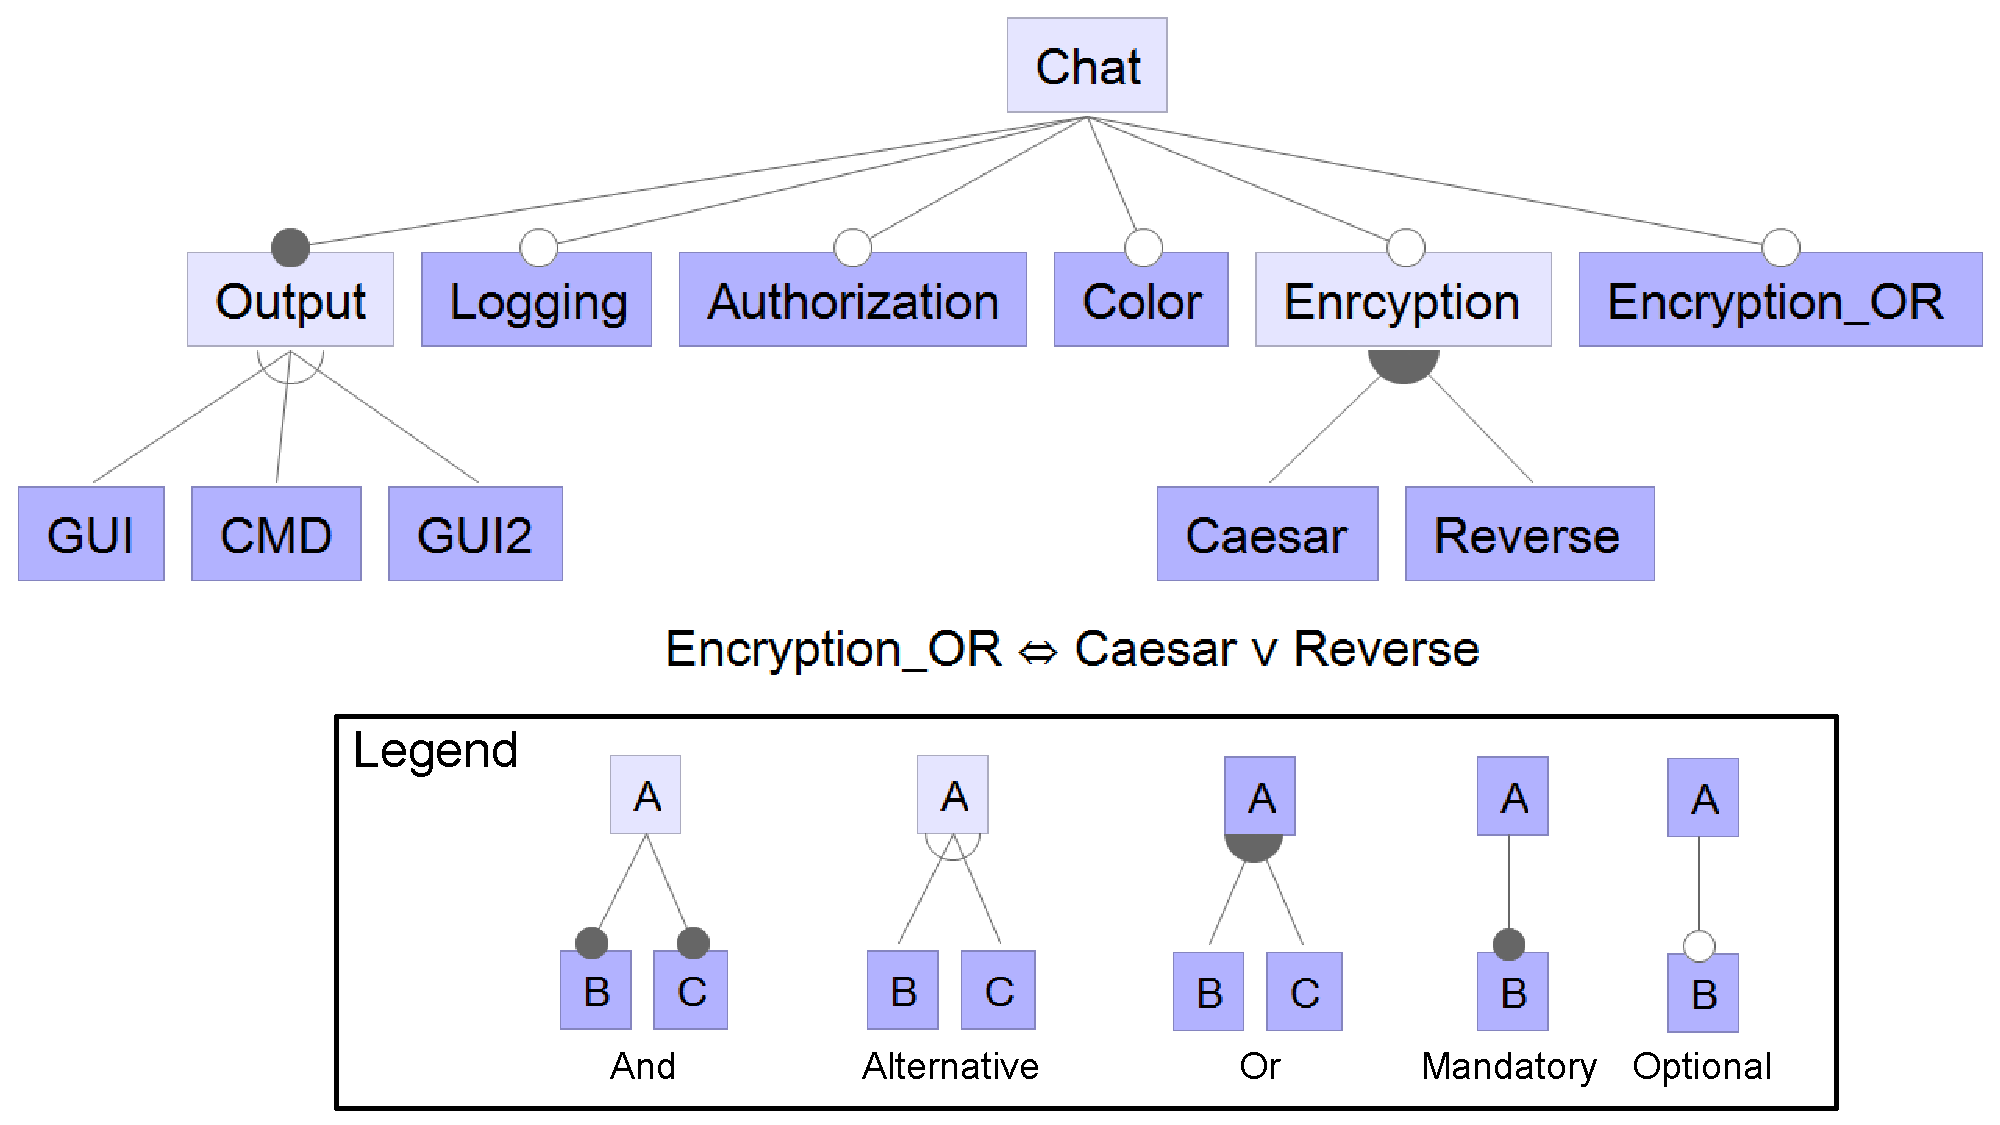
\epsfig{file=image/fm.bmp, width=8.5cm}
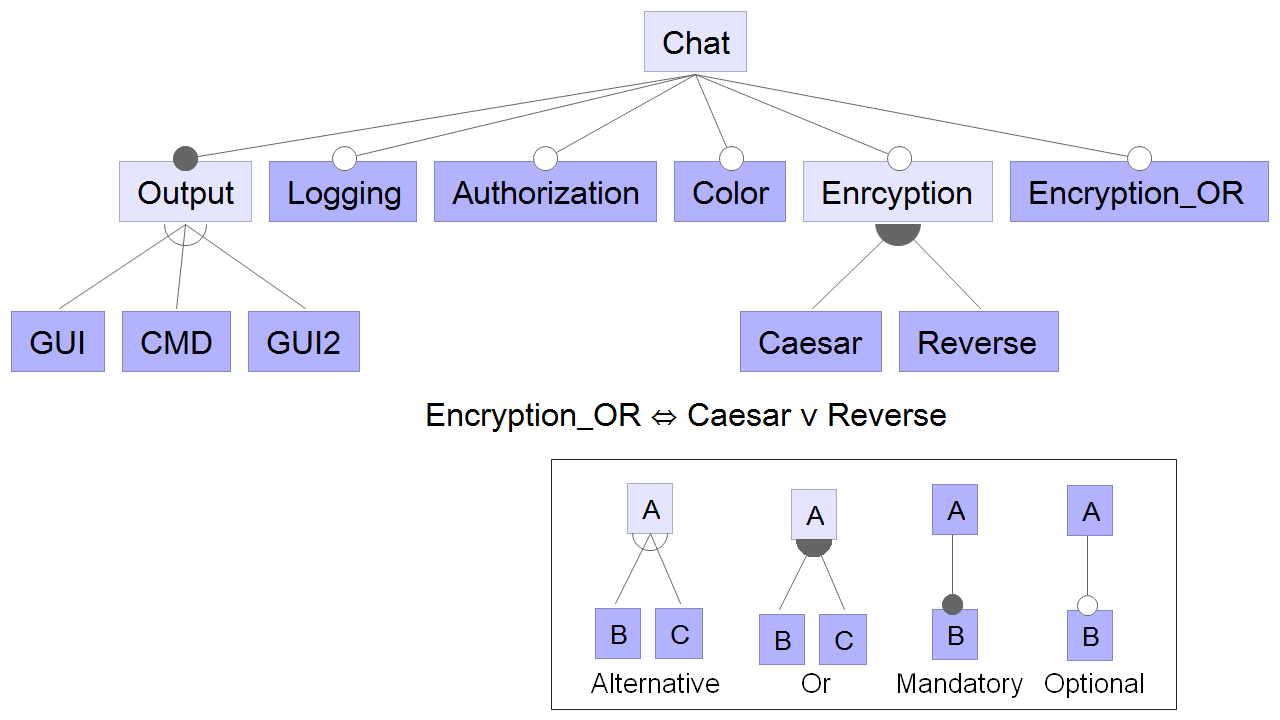
\includegraphics[width=8.5cm]{image/fm2.png}
\vspace{-2mm}
\caption{The feature model of $\JCS$ from \cite{DBLP:conf/issta/TanXCSLD15}}

\label{fig:re}
\end{figure}

The feature model of a Java Chat System ($\JCS$) is illustrated in Fig. \ref{fig:re} and the constraints of that model are listed in Table \ref{table:constrains}.
 Constraints c(1) -- c(12) are TCs, as they are constraints on structural relation of features. The root (compulsory) feature of the feature model is \textit{Chat}, which has a mandatory subfeature (\textit{Output}) and several optional subfeatures (e.g., \textit{Encryption}) --- constraints c(1) -- c(7). Since the feature \textit{Output}  is mandatory, exactly one of its subfeatures (\textit{GUI}, \textit{CMD}, and \textit{GUI2}) must be selected --- constraints c(8) -- c(11). In addition, if feature \textit{Encryption}  is selected, at least one of its subfeatures (\textit{Caesar} and \textit{Reverse}) needs to be selected --- constraints c(12). There is only one CTC for $\JCS$, which is of the form $f_1\ \mathit{iff}\ f_2$, \textit{Encryption\_OR} is selected if and only if \textit{Caesar} or \textit{Reverse} is selected ---  constraints c(13).

%The feature model listed in Fig. \ref{fig:re} can be captured by the constraints that are listed in~\mtable{table:constrains}. The constraints are specified according to the semantics of feature model.  %Constraint c(1) specifies that the root feature must be present, to prevent a trivial feature model with no selected feature. Constraint c(2) specifies the mandatory feature \textit{Output} and constraints c(3) -- c(7) specify constraints on the other five optional subfeatures. The subfeatures of \textit{Output} are in an \textit{Alternative} relationship. This is specified using constraints c(8) -- c(11). Constraint c(8) states that \textit{Output} is selected, if and only if at least one of \textit{CMD}, \textit{GUI} and \textit{GUI2} is selected. Constraints c(9) -- c(11) specify that at most one feature from \textit{CMD}, \textit{GUI} and \textit{GUI2} can be chosen. The subfeatures of \textit{Encryption} are in \textit{Or} relationship. The constraint c(12) denotes if \textit{Encryption} is selected, then at least one feature from \textit{Caesar} and \textit{Reverse} needs to be selected, and vice versa.
%The only CTC of $\JCS$ is captured in the constraint c(13).
Given a feature model \emph{M}, we refer TCs and CTCs of \emph{M} as  the conjunction of constraints of $M$, denoted by $\mathit{conj(M)}$. Let $\mathit{Fea(M)}$ denote the feature set of $M$, $\mathit{Fea(JCS)} = \{\scriptsize{\mathit{Chat}, \mathit{Output}, \mathit{Logging}, \mathit{Authorization}, \mathit{Color}, \mathit{Encryption},} \\ \scriptsize{\mathit{Encryption\_OR}, \mathit{GUI}, \mathit{CMD}, \mathit{GUI2}, \mathit{Caesar}, \mathit{Reverse}}\}$.% and $\mathit{\vert Fea(JCS) \vert}$=12.

%Given a feature model $M$,
%a \emph{feature valuation} is a function
%$\FV : \mathit{Fea(M)} \rightarrow \{\mathit{true}, \mathit{false}\}$ mapping a boolean value to each feature in the feature set $\mathit{Fea(M)}$, where the true (resp., false) value denotes the presence (resp., absence) of the feature. Given a constraint $C$, $C[\FV]$ denotes the constraint obtained by replacing each feature $Fea(M)$ with $\FV(F)$ in $C$.


%We write $\FV \models C$, if $C[\FV]$ evaluates to true, otherwise we write $\FV \not\models C$.

%  In addition to the tree constrains, there might be inter-feature cross-tree constrains (CTCs) like \textit{requires}, \textit{excludes} or \textit{iff}. In Figure \ref{fig:re}, below the feature model is a \textit{iff} type of CTCs c(12).

%In a feature model, a place that allows the flexible feature selection is called a variation point (VP) \cite{DBLP:conf/icsr/WebberG02}\cite{DBLP:conf/icse/JarzabekZLXS09}. The VP of a optional feature allows two options. The VP of an alternative relation of $n$ subfeatures allows $n$ options, while the VP of an or relation of $n$ subfeatures allows the options $C_{n}^{n} + C_{n}^{n-1}+ ...+ C_{n}^{1}$. Besides,

%A product derived from the feature model in Figure \ref{fig:re} must satisfy all constraints in Table \ref{table:constrains}. Therefore, finding a valid product derivation from a feature model can be reduced to a satisfaction problem on a set of logic formulas, also a NP-complete problem \cite{DBLP:journals/jss/WhiteDS09}. If the user preference values (extra non-functional constrains) are considered, finding an optimal product is shown to be NP-hard \cite{DBLP:conf/icse/SayyadMA13}. %\tth{Maybe just use a reference mentions that our work is NP-hard}

\vspace{-1mm}
\begin{myDef} [Correct  Solution]
Given a feature model $M$,  a \emph{correct solution}   for $M$ refers to a non-empty feature set $F \subseteq Fea(M)$ that satisfies the constraints of $M$.
\end{myDef}
\vspace{-1mm}

%We write $F \models M$ if $F \subseteq Fea(M)$ is a feasible feature set of the feature model $M$.
%\paratitle{Example}  We use
Take $\JCS$ as an example, $F=\{\mathit{Chat},\mathit{Output}, \mathit{GUI}\}$ is a correct solution of feature selection for $\JCS$. %Hence, an optimal feature selection must be a correct feature selection, and meanwhile, it optimizes several goals of product configuration.


%{\color{red} do you want to introduce the grammar of FM in this subsection or in the approach: the propositional logics for the semantic and constrains in FM?}

%Figure \ref{fig:re} shows the feature model of an SOSPL for online flight booking systems. This SOSPL can derive the different online flight booking system as a coarse-grained service to a different user. The \textit{abstract feature} in Figure \ref{fig:re} means this feature requires no specific implementation (thus, no need to be bound to a specific service), as an abstract feature usually is only a wrap of its sub-features. The \textit{concrete feature} means it has a specific function to perform, and it needs to be bound to a service to implement such function. Thus, in a valid product from this SOSPL, the selected concrete features must be bound to some services. Under the feature diagram in Figure \ref{fig:re}, the cross tree constrains of this FM are also listed.


\begin{table}[t]
\centering
\caption{Constraints of $\JCS$}
\vspace{-2mm}
\scalebox{0.9}{
\begin{tabular}{l|r}
\hline
$\mathit{Chat}$ & c(1)\\
$\mathit{Output} \iff  \mathit{Chat}$ & c(2)\\
$\mathit{Logging} \implies \mathit{Chat}$ & c(3)\\
$\mathit{Authorization} \implies \mathit{Chat} $ & c(4)\\
$\mathit{Color}\implies \mathit{Chat}$ & c(5)\\
$\mathit{Encryption}\implies \mathit{Chat}$ & c(6)\\
$\mathit{Encryption\_OR}\implies \mathit{Chat}$ & c(7)\\
$(\mathit{GUI} \lor \mathit{CMD} \lor \mathit{GUI2})\iff \mathit{Output}$ & c(8)\\
$\lnot(\mathit{GUI}\land \mathit{CMD})$ & c(9)\\
$\lnot(\mathit{GUI}\land \mathit{GUI2})$ & c(10)\\
$\lnot(\mathit{CMD}\land \mathit{GUI2})$ & c(11)\\
$(\mathit{Caesar}\lor \mathit{Reverse})\iff \mathit{Encryption}$ & c(12)\\
$\mathit{Encryption\_OR}\iff  (\mathit{Caesar} \lor \mathit{Reverse})$ & c(13)\\
\hline
\end{tabular}
}
%\vspace{-2mm}
\label{table:constrains}
\end{table}

\vspace{-1mm}
\subsection{Multi-objective Optimization for SPL}\label{sec:background:mop}
%Many real-world problems have multiple objectives that need to be optimized simultaneously. However, these objectives usually conflict with each other, which prevents optimizing all objectives simultaneously. A remedy is to have a set of optimal trade-offs between the conflicting objectives.

%A $k$-objective optimization problem could be written in the following form:
%\begin{equation}\label{eq:min}
%\begin{split}
%\emph{Minimize}\ Obj(F)=(Obj_1(F), Obj_2(F),..., Obj_k(F))\ \\  \emph{subject}\ \emph{to}\ F \models M
%\end{split}
%\end{equation}
%
% \noindent where $Obj(F)$ is a $k$-dimensional objective vector for $F$ and  $Obj_i(F)$ is the value of $F$ for $i$th objective.
%
%
%  Given $F_1, F_2 \models M$, $F_1$ can be viewed as better than $F_2$ for the minimization problem in~\mequation{eq:min}, if~\mequation{eq:minbetter} holds.
%
%A $k$-objective optimization problem could be written in the following form~\cite{abraham2005evolutionary}:
%\begin{equation}\label{eq:min}
%\emph{Minimize}\ f(x)=(f_1(x), f_2(x),..., f_k(x))\  \emph{subject}\ \emph{to}\ x \in X
%\end{equation}
%
%\noindent where $f(x)$ is a $k$-dimensional objective vector, and  $f_i(x)$ is the $i$th objective to be minimized, $x$ is the decision vector, and $X$ is the feasible region in the decision space.
%
%Consider $y$ and $z$ as two feasible solutions of the $k$-objective optimization problem in~\mequation{eq:min}, $y$ can be viewed as better than $z$ for the minimization probelm in~\mequation{eq:min}, if~\mequation{eq:minbetter} holds.

%\begin{equation}\label{eq:minbetter}
%\forall i: Obj_i(F_1) \leq Obj_i(F_2) \land \exists j: Obj_j(F_1) < Obj_j(F_2)
%\end{equation}
%
%\noindent  where $i,j \in \{1, \ldots, k\}$.
%
%In such a case, we say that $F_1$ \emph{dominates} $F_2$.  $F_1$ is called a \emph{Pareto-optimal solution} if $F_1$ is not dominated by any other $F \models M$. We denote all Pareto-optimal solutions as the \emph{Pareto front}.


%
% Assume $\textbf{y}$ and $\textbf{z}$ are two feasible solutions of the $k$-objective optimization problem, $\textbf{y}$ \emph{dominates} $\textbf{z}$ if $\forall i: f_i(\textbf{y}) \le f_i(\textbf{z})$ and $\exists j: f_j(\textbf{y}) < f_j(\textbf{z})$ where $i,j \in [1,k]$~\cite{DBLP:conf/gecco/IshibuchiTSN10}.
%
%
% $\textbf{y}$ is a \emph{Pareto-optimal solution} if $\textbf{y}$ is not dominated by any other feasible solutions. All Pareto-optimal solutions form the tradeoff space in the objective space, we denote the tradeoff space as the \emph{Pareto front}.


%To serve as the goals of malware generation, we propose three objective functions in the evolution of malware: \emph{aggressiveness}, \emph{evasiveness} and \emph{detectability}. As the results of the arms race, malware are getting more aggressive with minimum evasion features needed, but less detectable.
\subsubsection{Software Development Model and the Objectives}
As the correct selection of a non-empty feature set $F$ on feature model $M$ is essentially a boolean satisfiability (SAT) problem that attracted attention from researchers \cite{DBLP:conf/pfe/MannionC03}\cite{DBLP:conf/caise/BenavidesTC05}. %Insofar, many techniques have been applied to address this problem, such as theorem proving \cite{DBLP:conf/pfe/MannionC03}, Constraint Satisfaction Problems (CSP)~\cite{DBLP:conf/caise/BenavidesTC05} and OWL DL~\cite{DBLP:journals/ws/WangLSZP07}.
Gradually, this problem evolves into a MOO problem --- more than having a correct selection, multiple quality attributes of the product  generated according to $F$ need to be  optimized .

According to \cite{DBLP:journals/misq/Abdel-HamidSS99}, goals in software development indeed have a positive impact for the products. Project managers control the software development according to four objective scores: project risk; development cost, development defects; and manpower (total months of development)~\cite{DBLP:journals/misq/Abdel-HamidSS99}. %During product configuration for certain customers, project managers also consider other goals such as the richness of features and cost \cite{DBLP:conf/icse/SayyadMA13}.
According to \cite{DBLP:conf/icse/SayyadMA13}, each feature %(also with its relevant implementation module) in the feature model
is associated with three attributes, i.e., COST, DEFECT and USED\_BEFORE. The optimal feature selection problem can be ideally modeled as a MOO problem, which requires trade-off among multiple design goals.

\subsubsection{Formalization of the MOO Problem}\label{sec:problem:moo}

  Given a non-empty feature set $F$ and the entire feature set $Fea(M)$ for $M$ ($Fea(M) =\{f_1 ... f_n\}$. For  $ \forall f_i \in Fea(M)$, the binary value represented by the selection of $f_i$ (denoted as $|f_i|$) is \textbf{1} if $f_i \in F$, else $|f_i|$ is  \textbf{0}. Given a solution $\vec x$ (an encoded binary-value vector for $Fea(M)$),  we define objective functions as:

%\footnote{For the sake of simplicity and ease of evaluation, we use the five objectives defined in \cite{DBLP:conf/icse/SayyadMA13} for problem statement and evaluation.}
\begin{enumerate}[label=\textbf{Obj\arabic*.},itemindent=*]
  \item \textbf{Correctness} means the extent of the compliance to $conj(M)$. We want to minimize the number of violated constraints:  $\mathcal{F}_1(\vec x) = Viol(F)$, where $Viol(F)$ returns the number of constraints violated by $F$ among $conj(M)$. Note that $Viol(F)$ = 0 means a  correct selection.
  \item  \textbf{Richness of features} means the richness of the functionality of the product. We want to minimize the number of deselected features: $\mathcal{F}_2(\vec x) = \sum\nolimits_{i=1}^{n} (1-|f_i|)$, where $|f_i|$ returns 1 if $f_i \in F$, otherwise returns 0.
  \item   \textbf{Feature used before} means the reliability of product, as features never used are more prone to have unknown defects. We want to minimize this:
      $  \mathcal{F}_3(\vec x) = \sum\nolimits_{i=1}^{n} (Used(f_i)  \cdot  |f_i|)$, where $Used(f_i)$ returns a boolean value of the attribute USED\_BEFORE of feature $f_i$.
   \item \textbf{Defects} means the known bugs or errors contained in the product. We want to minimize this: %It can be quantified by the $
       $\mathcal{F}_4(\vec x) =  \sum\nolimits_{i=1}^{n}( Defect(f_i)   \cdot  |f_i|)$, where $Defect(f_i)$ returns the value of attribute DEFECT of feature $f_i$.
  \item  \textbf{Cost} means the expense and efforts in developing the product. We want to minimize this: $\mathcal{F}_5(\vec x) = \sum\nolimits_{i=1}^{n}( Cost(f_i)  \cdot   |f_i|)$, where  $Cost(f_i)$ returns the value of the attribute COST of feature $f_i$.
\end{enumerate}

%\vspace{-2mm}
%\begin{myDef}\label{def:aggressivity}
% \textbf{Correctness} means the extent of compliance to the relationships and constraints contained in the feature model, and can be formally defined as follow %such as privacy leakage, resource depletion, or controlled as a bot.  and the set of selected attack features $S_a$, aggressivity $f_1(x)$ is defined as follows:
%     \begin{equation}
%       \mathcal{F}_1(x) = Corr(F)
%         \end{equation} where $Corr(F)$ returns the number of violated constraints of $F$ among all the constraints of $M$\footnote{Note that $Corr(F)$ = 0 means that $F$ produces a correct feature selection.}.
%         %It can be measured by  the number of attack features contained in malware.
%       %It can be quantified by the number of contained attack features.
%\end{myDef}
%\vspace{-2mm}
%\vspace{-2mm}
%\begin{myDef}\label{def:complexity}
%\textbf{Richness of features} means the richness of the functionality of the product. It is measured by the number of selected features and defined as follows
%        \begin{equation}
%         \mathcal{F}_2(x) = \sum\nolimits_{i=1}^{n} \|f_i\|
%           \end{equation} where $\|f_i\|$ returns 1 if $f_i$ is selected and returns 0 if not.
%        %It can be measured by the number of evasion features used by malware. %It can be quantified by the number of used evasion features.\
%\end{myDef}
%\vspace{-2mm}
%
%%Given a chromosome $x$ and the set of AMTs $S_d$, $\{d_1...d_t\}$, introduced in Section \ref{sec:defense}, we have the following definition for the last objective function:
%
%\begin{myDef}\label{def:complexity}
%\textbf{Cost} means the expense and efforts in developing the product. It is an aggregate value and defined as follows
%        \begin{equation}
%         \mathcal{F}_3(x) = \sum\nolimits_{i=1}^{n}( Cost(f_i) \cdot   \|f_i\|)
%           \end{equation} where  $Cost(f_i)$ returns the value of the attribute COST of feature $f_i$.
%        %It can be measured by the number of evasion features used by malware. %It can be quantified by the number of used evasion features.\
%\end{myDef}
%\vspace{-2mm}
%
%\begin{myDef}\label{def:complexity}
%\textbf{Feature used before} means the reliability of product, as the features never used are more prone to contain unknown defects. It is an aggregate value and defined as follows
%        \begin{equation}
%         \mathcal{F}_4(x) = \sum\nolimits_{i=1}^{n} (Used(f_i)  \cdot  \|f_i\|)
%           \end{equation} where $Used(f_i)$ returns the boolean value of the attribute USED\_BEFORE of feature $f_i$.
%        %It can be measured by the number of evasion features used by malware. %It can be quantified by the number of used evasion features.\
%\end{myDef}
%\vspace{-2mm}
%
%\vspace{-2mm}
%\begin{myDef}\label{def:detectability}
% \textbf{Defects} means the bugs or errors contained in the product. It is an aggregate value and defined as follows  %It can be quantified by the detection ratio by different malware detection tools.
%       \begin{equation}
%       \mathcal{F}_5(x) =  \sum\nolimits_{i=1}^{n}( Defect(f_i)  \cdot  \|f_i\|)
%       \end{equation} where $Defect(f_i)$ returns the value of attribute DEFECT of feature $f_i$.
%\end{myDef}
%\vspace{-2mm}

%\subsubsection{Generation Steps}
%\vspace{-2mm}

%Since DSA capture the essence of malicious behaviors (see Chapter~\ref{sec:model}), we first construct basic malicious behaviors in terms of these DSA, then instrument communication mechanisms existing in Android to the malicious behaviors, and last employ obfuscation techniques to instrument the malware. The malware is sent to the module of risk assessment, which can give its fitness. The process is iterative and the malware evolves according to the fitness feedback. In this chapter, we elaborate the steps of malware generation.

%In this section, we introduce the algorithm to select the features, and improve the feature combination according to the evaluation of generated apps.

Rather than encode all the objectives into one magic weighted fitness function, all the objectives are equally treated and solved by MOO using the Pareto dominance relation~\cite{mopsurvey2008}.


A $k$-objective optimization problem could be written in the following form %\footnote{\small Evasiveness and detectability need to be minimized, but aggressiveness needs to be maximized. In implementation, maximizing is minimizing the negative value of the objective.}
(in our case, $k = 5$):
\begin{equation}\label{eq:min}
\begin{split}
\emph{Minimize}\ \mathcal{\vec F}=(\mathcal{F}_1(\vec x), \mathcal{F}_2(\vec x),..., \mathcal{F}_k(\vec x))\ \\ % \emph{subject}\ \emph{to}\ F \models M
\end{split}
\end{equation}
\noindent where $\mathcal{\vec F}$ is a $k$-dimensional objective vector and  $\mathcal{F}_i(\vec x)$ is the value of $\mathcal{\vec F}$ for $i$-th objective.
\begin{myDef}
Given two correct solutions $\vec x, \vec y \in B^n$ and an objective vector $ \mathcal{\vec F}: B^n \rightarrow R^k$, $\vec x$ \textbf{dominates} $\vec y$ ($ \vec x \prec \vec y$) if
    \begin{equation}
    \begin{split}
  \forall i \in \{1,...,k\} \quad \mathcal{F}_i(\vec x) \le \mathcal{F}_i(\vec y)
  \end{split}
     \end{equation}
    \begin{equation}
     \begin{split}
   \exists j \in \{1,...,k\} \quad \mathcal{F}_j(\vec x) < \mathcal{F}_j(\vec y)
     \end{split}
   \end{equation}
otherwise $\vec x \not\prec \vec y$
\end{myDef}
\vspace{-2mm}

\vspace{-2mm}
\begin{myDef}
Given a correct solution $\vec x$ and a set of correct solutions $S_{\vec x}$, $\vec x$ is \textbf{non-dominated} iff
      \begin{equation}
  \forall \vec x_i \in S_{\vec x} \quad \vec x_i \not\prec \vec x
       \end{equation}
\end{myDef}
\vspace{-2mm}
$\vec x$ is called a \emph{Pareto optimal} solution if $\vec x$ is \emph{correct} and \emph{not dominated} by any other correct solutions. All Pareto-optimal solutions are called as the true Pareto front.

\subsubsection{Problem Statement}

%\paratitle{Problem statement}
Existing MOEAs (e.g., IBEA~\cite{DBLP:conf/ppsn/ZitzlerK04}, NSGA-II~\cite{DBLP:journals/tec/BradstreetWB08}, ssNSGA-II~\cite{coello2004applications}, MOCell~\cite{miettinen1999nonlinear}, SPEA2 \cite{Zitzler01spea2:improving})  are used to find a set of non-dominated solutions that approximate the Pareto front for solving the MOO problems. %According to \cite{DBLP:conf/icse/SayyadMA13}, among them, NSGA-II and SPEA2 are most widely used in SBSE. For the optimal feature selection problem,
As pointed by Sayyad \emph{et.al} in \cite{DBLP:conf/icse/SayyadMA13}, IBEA produces the solutions with the highest correctness rate. After that, more studies improve IBEA to search for correct solutions \cite{conf/cmsbse/SayyadMA13}\cite{DBLP:conf/issta/TanXCSLD15}\cite{DBLP:conf/icse/HenardPHT15}\cite{DBLP:journals/tosem/HieronsLLSZ16}\cite{DBLP:journals/asc/XueZT0CC016}.

%However, whatever MOEA is used, the completeness of the found solutions and the quality of the approximated Pareto front cannot be guaranteed.

%\paratitle{Motivation}
%Our work addresses the \emph{optimal feature selection}. Nevertheless,
 As these MOEA-based approaches suffer from the correctness, %we treat this optimal feature selection problem as a mix of SAT and MOO problem ---  assure the solutions are correct solutions (i.e., assuring $Vio(F)=0$) and then optimize the other four objectives.
why not we use a method naturally assuring the solution correctness?   As all constraints in $conj(M)$  and all objectives are \emph{linear} (convertible to linear inequalities, see \S\ref{sec:formulate}),  Binary Integer Programming (BIP) can be applied. In theory, we can reduce the multiple objectives into one. The BIP-based analytic method is free from the drawbacks of MOEAs (see \S\ref{sec:intro}), but may suffer from the scalability issue. %In \S\ref{sec:naiveSolutions} and \S\ref{sec:solution}, we reduce multi-objective to one for applying LP.

%it is \xyx{Inspired by [??], we aim to design an analytic approach that solve the subproblem of satisfiability and  optimisation subproblem  in polynomial time. }

 %, such as Genetic Algorithms, Evolutionary Strategies and Differential Evolution.

%We use the Indicator-Based Evolutionary Algorithm (IBEA)~\cite{DBLP:conf/ppsn/ZitzlerK04}, which has already been implemented in the jMetal framework~\cite{DBLP:journals/aes/DurilloN11}.
%\subsection{Problem Statement}


%Given multiple objectives to be optimized, we have the following definition:

%\begin{definition} [optimal feature set]
%Given a feature model $M$,  an \emph{optimal feature set} for $M$ is a feasible feature set $f \models M$, which is not dominated by any feasible feature set $f' \models  M$, where $f \neq f'$.
%\end{definition}

%\begin{definition}[optimal feature selection]
%Given a feature model $M$,  an \emph{optimal feature selection} is a set of optimal feature sets of $M$.
%\end{definition}
%\emph{Optimal feature selection} of feature model $M$ is to select a set of optimal features sets for $M$.

%Our work addresses \emph{optimal feature selection}, which aims to search for a feasible feature sets that approximate the Pareto
%front for solving the multi-objective optimization problem.

%We denote the \emph{size} of optimal feature selection $S$ as the number of optimal feature sets in $S$.

%In addition, given two EAs $ea_1$ and $ea_2$, we say that $ea_1$ provides an improvement than $ea_2$ in finding an optimal feature selection, if the size of the optimal feature selection found by $ea_1$ is strictly larger than $ea_2$.

%\paratitle{Example} We use $\JCS$ as an example. Suppose we want to minimize the cost of the feature selection, and all features are free, except features $\mathit{GUI}$ comes with a cost. In this case, $f=\{\mathit{Chat},\mathit{Output},\mathit{GUI}\}$ is a feasible feature selection, but it is not an optimal feature selection. This is because $f$ is dominated by, for example $\{\mathit{Chat},\mathit{Output},\mathit{CMD}\}$, which has lower cost. Both $o_1=\{\mathit{Chat},\mathit{Output},\mathit{CMD}\}$ and $o_2=\{\mathit{Chat},\mathit{Output},\mathit{GUI2}\}$ are optimal feature sets, and $\{o_1, o_2\}$ is an optimal feature selection, with size of 2.


\section{Mathematical Formulation of the Problem}\label{sec:formulate}
%Software companies that maintain an SPL want to respond to the various market and customers rapidly, while still considering a large amount of features and constraints among the features.
To apply IP methods, logical formulae shown in Table \ref{table:constrains} are converted into inequalities to serve as linear constraints in IP.  %An internationally accepted and widely applied standard

\subsection{Theory of Converting Logical Formulae to Inequalities}\label{sec:convert}
Converting logical formulae (LF) into inequalities is a typical problem of OR. By BIP upon the inequalities, it can be rapidly decided whether the original given LFs can be satisfied and how to be satisfied if so.
In \cite{Hooker:1988}, Hooker proposed and proved that the satisfiability problem of a conjunctive normal form (CNF) can be directly reduced to a BIP problem.
Though detailed steps are not formalized in \cite{Hooker:1988}, the basic idea of conversion was explained. %First, any arbitrary logical formula should be represented as a conjunction of \emph{1-clause}, namely \emph{clause of degree one}. Here, \emph{clause of degree} $\beta$ asserts that there are at least $\beta$  literals (corresponding to variables in BIP) to be true.
%Second,
Generally, two ways can convert an arbitrary LF as a CNF. Except for each atomic proposition, if no extra variables are introduced for operations on several atomic propositions, the running time and length of the resulting CNF can increase exponentially with the number of atomic propositions in the original formula in the worse case \cite{DBLP:journals/cor/BlairJL86}. %But if with extra variables, the conversion can finish in linear time .
%all the formulae in a system constitute the knowledge base, which is the conjunction of its formulae. For instance, constraints (1) to (13) in Table \ref{table:constrains} constitute the knowledge base of the model \emph{JCS}.

\subsection{Fast Converting Logical Formulae from the SPL Models}\label{sec:convert}
As different types of TCs and CTCs are actually not arbitrary LFs, the conversion can be done in linear time without introducing intermediate CNFs and extra variables. Let $|f_i|$ denote whether the $i$-th feature ($f_i$) is selected in a solution (see \S\ref{sec:background:mop}). We can deduce the following lemmas:
%Owing to the specific types of constraints in SPL models, the constraints are actually not arbitrary logic formulae. In this case, can the conversion be done in linear time even without introducing extra variables? The answer is yes. It is unnecessary to represent all TCs and CTCs as CNFs.

 %Different types of TCs and CTCs can be readily converted into inequalities  without introducing intermediate CNFs and extra variables. $|f_i|$ --- whether the $i$-th feature is inside the set of selected features  $F$  from $Fea(JCS)$ (see \S\ref{sec:background:mop})

\begin{lem}\label{lem:optional}If feature $f$ is an Optional subfeature  of feature $f^\prime$, the linear inequality for the Optional relationship is
  \begin{equation}
  |f^\prime| - |f| \ge 0
  \end{equation}
  \end{lem}
\begin{proof}
  $f \Rightarrow f^\prime$  is \emph{true} according to the optional relationship. Thus we can infer $\neg f  \lor f^\prime$  is \emph{true}. As a CNF, it can be converted to the inequality $(1-|f|)+|f^\prime| \ge 1$, that is $  |f^\prime| - |f| \ge 0$.
\end{proof}

\vspace{-3mm}
\begin{lem}\label{lem:mandatory}
If feature $f$ is a Mandatory subfeature  of feature $f^\prime$, the linear equality for the Mandatory relationship is
  \begin{equation}
  |f^\prime| - |f| = 0
  \end{equation}
\end{lem}
\begin{proof}
  $f \Leftrightarrow f^\prime$ is \emph{true} according to the mandatory relationship. Thus we infer the CNF $ (\neg f  \lor f^\prime) \land ( \neg  f^\prime \lor  f)$  is \emph{true}. Two inequalities are deduced:  $(1-|f|)+|f^\prime| \ge 1$ and $(1-|f^\prime| )+ |f|\ge 1$. By unifying them, we infer $|f^\prime| - |f| = 0$.
\end{proof}

\vspace{-2mm}
\begin{lem}If features $f_1$ ... $f_n$ are  the Or-subfeature of feature $f^\prime$, %the  equality for the Or relationship is
%  \begin{equation}
%  \prod\nolimits_{i=1}^{n}{(1- f_i)} + f^\prime  = 1
%  \end{equation}
%\noindent and
the linear inequalities for this relationship are
  \begin{equation}
  \forall  i \in  \{1,...,n\}, ~~ |f_i| -  |f^\prime|  \le 0  \label{formula:or1}
  \end{equation}
  \begin{equation}
  \sum\nolimits_{i=1}^{n}{|f_i|} - |f^\prime| \ge 0 \label{formula:or2}
  \end{equation}
\end{lem}
\begin{proof}
$\bigvee\nolimits_{i=1}^{n}({f_i})  \Leftrightarrow f^\prime $ is \emph{true} according to the Or relationship. Here, $\bigvee\nolimits_{i=1}^{n}({f_i})$ notates $f_1 \lor f_2 \lor ... \lor f_n $. Thus, the formulae $\bigvee\nolimits_{i=1}^{n}({f_i})  \Rightarrow f^\prime $ and $f^\prime \Rightarrow \bigvee\nolimits_{i=1}^{n}({f_i})$ need to be \emph{true}. For the first formula, we can represent it as the CNF and get the resulting formula $\bigwedge \nolimits_{i=1}^{n}({\neg f_i \lor f^\prime})$  to be \emph{true}. Note that for an indexed set of propositions $P = \{p_1,...,p_n\}$, $\bigwedge\nolimits_{i=1}^{n}(p_i)$ means that each proposition in $P$ needs to be \emph{true}.  Thus, we can get $n$ derived linear  inequalities that are listed in the inequality (\ref{formula:or1}). For the second formula $f^\prime \Rightarrow \bigvee\nolimits_{i=1}^{n}({f_i})$, we get $\neg f^\prime \lor \bigvee\nolimits_{i=1}^{n}({f_i})$ to be \emph{true}, that is $ \neg f^\prime \lor f_1 \lor ... \lor f_n $ to be true. So the inequality   (\ref{formula:or2}) can be deduced from the second formula.
\end{proof}



\begin{lem}If features $f_1$ ... $f_n$ are the Alternative subfeature of feature $f^\prime$, the linear inequalities for this relationship are
  \begin{equation}
  \forall  i \in  \{1,...,n\}, ~~ |f_i| -  |f^\prime|  \le 0
  \end{equation}
  \begin{equation}
  \sum\nolimits_{i=1}^{n}{|f_i|} - |f^\prime| \ge 0
  \end{equation}
  \vspace{-4mm}
  \begin{equation}
  \sum\nolimits_{i=1}^{n}{|f_i|}  \le 1 \label{formula:alter3}
  \end{equation}
  \end{lem}
\begin{proof}
Essentially, alternative subfeatures are a special type of \emph{or} features. In the subfeatures of an \emph{or} relationship, at least one subfeature needs to be selected. Whereas, only and exactly one needs to be selected in the alternative subfeatures. Instead of using inequalities  c(9)--c(11) in Table \ref{table:constrains}, the concise inequality (\ref{formula:alter3}) is  used to assure the exclusiveness of all subfeatures.
\end{proof}
Except the above 4 types of TCs, there are 3 types of CTCs. The \emph{requirement} of $f^\prime$ for $f$ can be formulated as $f \Rightarrow f^\prime$, and we can deduce $|f^\prime|-|f| \ge 0$ according to Lemma \ref{lem:optional}. Similarly, the \emph{iff} relationship between $f^\prime$ and $f$ is formulated as $f \Leftrightarrow f^\prime$, and we can deduce  $|f^\prime| - |f| = 0$ according to Lemma \ref{lem:mandatory}. Last, we have the last type of CTCs:

\begin{lem}If feature $f$ Excludes feature $f^\prime$, the linear equality for the Exclusion relationship is
  \begin{equation}
   |f^\prime| + |f| \le 1
  \end{equation}
  \end{lem}
\begin{proof}
$f \Rightarrow \neg f^\prime$ is \emph{true} according to the exclusion relationship. Thus we can infer $\neg f  \lor \neg f^\prime$  is \emph{true}. As a CNF, it can be converted to $(1-|f|)+(1-|f^\prime|) \ge 1$, that is $  |f^\prime| + |f| \le 1$.
\end{proof}

\subsection{The Integer Programming Model of Our Example}\label{sec:spl_ip_problem}
Let $\vec x$ be a solution, a binary variable vector $\vec x \in \{0,1\}^n$  where variable $x_i$ denotes $|f_i|$.
For each feature $f_i$, we denote its attributes $Used(f_i)$, $Defect(f_i)$ and $Cost(f_i)$ as coefficient $a_i$, $b_i$ and $c_i$, respectively. We denote the objective function for $obj_j$ as $\mathcal{F}_j(\vec x)$, $j \in \{1,...,k\}$. Subject to the linear inequalities converted from TCs and CTCs,
the example is formulated  as a multi-objective BIP (MOBIP) problem:

\begin{equation}\label{formula:mop}
%%\begin{array}{rrclcl}
%%\displaystyle \min_{x} & \multicolumn{3}{l}{c^T x} \\
%%\textrm{s.t.} & A x & \geq & b \\
%%%&\displaystyle \sum_{i=0}^{n} x_i & = & 1 \\
%%& x_i & \in & \{0,1\} & & \forall i \in \{1...n\} \\
\begin{array}{ll@{}r@{}r@{}l}
    \text{Min} & \mathcal{F}_2(\vec x)= \sum\nolimits_{i=1}^{n}(1-x_i) \\[\jot]
    \text{Min} & \mathcal{F}_3(\vec x)=\sum\nolimits_{i=1}^{n}(a_i\cdot x_i) \\[\jot]
    \text{Min} & \mathcal{F}_4(\vec x)=\sum\nolimits_{i=1}^{n}(b_i\cdot x_i) \\[\jot]
    \text{Min} & \mathcal{F}_5(\vec x)=\sum\nolimits_{i=1}^{n}(c_i\cdot x_i) \\[\jot]
    \text{s.t.} & \text{the inequalities for $conj(M)$ hold}\\[\jot]

%    &  x_1 - x_3  \ge 0   \\
%    &  x_1 - x_4 \ge 0      \\
%    &  x_1 - x_5 \ge 0      \\
%    &  x_1 - x_6 \ge 0      \\
%    &  x_1 - x_7 \ge 0      \\
%    &  x_2 - x_8 \ge 0      \\
%    &  x_2 - x_9 \ge 0      \\
%    &  x_2 - x_{10} \ge 0      \\
%    &  -x_2 + x_8 + x_9 + x_{10}\ge 0      \\
%    &  -x_8 - x_9 - x_{10}\ge -1      \\
%    &  x_6 - x_{11} \ge 0      \\
%    &  x_6 - x_{12} \ge 0      \\
%    &  -x_6 + x_{11} + x_{12} \ge 0      \\
%    &  x_7 - x_{11} \ge 0      \\
%    &  x_7 - x_{12} \ge 0      \\
%    &  -x_7 + x_{11} + x_{12} \ge 0      \\
  \end{array}
%%\end{array}
\end{equation}
%s.t. the inequalities for c(1)--c(13) in Table \ref{table:constrains} hold.\\

\section{$\epsilon$-constraint Method and CWMOIP}\label{sec:naiveSolutions}

When the problem size is relatively small, the $\epsilon$-constraint method and CWMOIP are two feasible methods to find the complete non-dominant solutions (a.k.a., true Pareto front).

\begin{algorithm}[t]
                  % enter the algorithm environment
\caption{Function \small{$EpsilonCont()$} for feature selection}\label{alg:naiveLP}
\small
    \KwIn{$M$: the feature model of the given system} %$maxIter$: the maximum number of iterations of the generation process
    %\KwIn{$userInfor$: the contextual information of user device} %$maxIter$: the maximum number of iterations of the generation process
    \KwOut{$solutions$: a non-dominated solution set for feature selection}
    %\KwOut{$returnedSol$: a solution returned to guide malware generation }
    $E~\leftarrow~\emptyset$\;\label{algo:lp:i1}
    $f^{TUB}_2 = getObjTheoBound(M,\mathcal{F}_2), f^{TLB}_2 = 0$\;\label{algo:lp:i2}
    $f^{TUB}_3 = getObjTheoBound(M,\mathcal{F}_3), f^{TLB}_3 = 0 $\;\label{algo:lp:i3}
    $f^{TUB}_4 = getObjTheoBound(M,\mathcal{F}_4), f^{TLB}_4 = 0 $\;\label{algo:lp:i4}

     \For{$ p=f^{TLB}_2;   p \le f^{TUB}_2; p = p \small{+} 1$}{\label{algo:lp:f1}
        \For{$ q= f^{TLB}_3;  q \le f^{TUB}_3; q = q\small{+} 1$}{\label{algo:lp:f2}
          \For{$ t=f^{TLB}_4;  t \le f^{TUB}_4; t = t\small{+} 1$}{\label{algo:lp:f3}
          %$conj(\mathcal{F}_2) = convert(\mathcal{F}_2,p) $\; \label{algo:lp:lp1}
          %$conj(\mathcal{F}_3) = convert(\mathcal{F}_3,q) $\; \label{algo:lp:lp2}
          %$conj(\mathcal{F}_4) = convert(\mathcal{F}_4,t) $\; \label{algo:lp:lp3}
          $allCons= conj(M) \cup \{\mathcal{F}_2\le p\} \cup \{\mathcal{F}_3\le q\}  \cup \{\mathcal{F}_4 \le t\} $\;\label{algo:lp:lp4}
          $ME = bintprog(allCons,\mathcal{F}_5) $\; \label{algo:lp:lp5}
          $E = E \cup ME$\;  \label{algo:lp:lp6}
          }
        }
     }
    % $returnedSol = solutions.First()$\;
   %  \For{$sol  \in  nondominatedSol$}{  \label{algo:lp:f3}
%        \If {$  aggregatedObj(sol) < aggregatedObj(returnedSol)$} {               \label{algo:lp:if1}
%       %  \If {$ satisfyExtraConst(sol) == true $} {               \label{algo:lp:if2}
%          $returnedSol = sol$\; \label{algo:lp:if3}
%       %   }
%        }
%     }

    \KwRet $E$;\label{algo:lp:rt}
      %  $allMal\leftarrow allMal \cup newGeneration$\;\label{algo:cmb:23}

\end{algorithm}

\subsection{$\epsilon$-constraint Method}
The idea is to make $k-1$ objectives as the range constraints and use the $k$-th one as the objective function in BIP \cite{e-constraint}. As \emph{obj1} is correctness, in BIP, all the constraints are satisfied, \emph{obj1} is always 0 in theory and thus $\mathcal{F}_1(\vec x)$ is not needed. So $\mathcal{F}_2(\vec x)$, $\mathcal{F}_3(\vec x)$, $\mathcal{F}_4(\vec x)$ can be converted to range constraints. Each range constraint's upper bound will be iterated from 0 to the upper bound of the corresponding objective, by step size 1.

The detailed procedures are shown in Algorithm \ref{alg:naiveLP}. Note that $getObjTheoBound(M,\mathcal{F}_2)$ at line \ref{algo:lp:i2} finds the theoretic upper bound $f^{TUB}_2$ for $\mathcal{F}_2$ --- for \emph{JCS}, it is 12 when all $x_i=0$  and $conj(M)$ is not considered. Similarly, $f^{TUB}_3$ and $f^{TUB}_4$ are $\sum\nolimits_{i=1}^{n}a_i$ and $\sum\nolimits_{i=1}^{n}b_i$ respectively,  when the size of feature set $n = \mathit{\vert Fea(JCS) \vert} =12$ for \emph{JCS}. At line \ref{algo:lp:lp4},  $allCons$ is the union of the original inequalities of the formula (\ref{formula:mop}) and three new inequalities converted from other constrained objectives in formula  (\ref{formula:singLP}). At line \ref{algo:lp:lp5}, $bintprog(allCons,\mathcal{F}_5)$ calls the BIP function for objective $\mathcal{F}_5$ such that $allCons$ are satisfied.

\vspace{-3mm}
\begin{equation}\label{formula:singLP}
%%\begin{array}{rrclcl}
%%\displaystyle \min_{x} & \multicolumn{3}{l}{c^T x} \\
%%\textrm{s.t.} & A x & \geq & b \\
%%%&\displaystyle \sum_{i=0}^{n} x_i & = & 1 \\
%%& x_i & \in & \{0,1\} & & \forall i \in \{1...n\} \\
\begin{array}{ll@{}r@{}r@{}l}
     \text{Min} & \mathcal{F}_5(\vec x) =\sum\nolimits_{i=1}^{n}(c_i\cdot x_i) \\[\jot]
     \text{s.t.} & \sum\nolimits_{i=1}^{n}(1-x_i) \le p \\[\jot]
      & \sum\nolimits_{i=1}^{n}(a_i\cdot x_i) \le q \\[\jot]
      & \sum\nolimits_{i=1}^{n}(b_i\cdot x_i) \le t\\[\jot]
       & \text{the inequalities for $conj(M)$ hold}\\[\jot]
%    &  x_1 - x_3  \ge 0   \\
%    &  x_1 - x_4 \ge 0      \\
%    &  x_1 - x_5 \ge 0      \\
%    &  x_1 - x_6 \ge 0      \\
%    &  x_1 - x_7 \ge 0      \\
%    &  x_2 - x_8 \ge 0      \\
%    &  x_2 - x_9 \ge 0      \\
%    &  x_2 - x_{10} \ge 0      \\
%    &  -x_2 + x_8 + x_9 + x_{10}\ge 0      \\
%    &  -x_8 - x_9 - x_{10}\ge -1      \\
%    &  x_6 - x_{11} \ge 0      \\
%    &  x_6 - x_{12} \ge 0      \\
%    &  -x_6 + x_{11} + x_{12} \ge 0      \\
%    &  x_7 - x_{11} \ge 0      \\
%    &  x_7 - x_{12} \ge 0      \\
%    &  -x_7 + x_{11} + x_{12} \ge 0      \\
  \end{array}
\vspace{-3mm}
%%\end{array}
\end{equation}

Algorithm \ref{alg:naiveLP} is of the time complexity of $O(n^3)$, if considering BIP solving function $bintprog()$ takes constant time --- a time limit is set in its practical usage. Solving the MOBIP problem in formula (\ref{formula:mop}) is reduced to solving the BIP problem in formula (\ref{formula:singLP}) by many times --- precisely, it is a number of $(n+1)  ({\sum\nolimits_{i=1}^{n}a_i}+1)({\sum\nolimits_{i=1}^{n}b_i}+1)$ times.



\subsection{CWMOIP}
CWMOIP, proposed by  \"{O}zlen \emph{et al.}~\cite{DBLP:journals/eor/OzlenA09}, is an objective-reduction technique for MOIP. CWMOIP is for generating \emph{all} non-dominant solutions.
It improves the $\epsilon$-constraint method by two steps: (1) for each objective, the lower bound is not 0 and the upper bound is not the sum of feature attributes revelent to that objective. To be precise, BIP is applied to get the true lower and upper bounds for each objective (i.e., $\mathcal{F}_2$ to $\mathcal{F}_5$) separately, subject to the  conjunction of constraints $conj(M)$. (2) objective-reduction is implemented via the constraint weight method, to avoid generating dominant solutions. The $k$-objective problem is first reduced to that of $k-1$, then $k-2$, iteratively, until the last objective.

\noindent\textbf{Example for (1).} In the precise calculation of the upper and lower bounds, for the example of \emph{JCS} with 12 features, the true bounds $f^{LB}_2$ and $f^{UB}_2$ for $\mathcal{F}_2(\vec x)$ are 2 (a maximum of 10 selected  features) and 9 (a minimum of 3 selected) respectively, not 0 and 12 in the $\epsilon$-constraint method. Hence, in $\epsilon$-constraint method 13 (12-0+1) times of iteration is needed for the outermost loop at line~\ref{algo:lp:f1} in Algorithm \ref{alg:naiveLP}, while  only 8 (9-2+1) times is needed for CWMOIP.


\begin{algorithm}[t]                  % enter the algorithm environment
\caption{Function \small{\emph{CWMOIP()}} for $k$-objective IP}\label{alg:cwmoip}
\small
    %\KwIn{$M$: the feature model of the given system} %$maxIter$: the maximum number of iterations of the generation process
    \KwIn{$k$: the number of objectives, $l_k$: constrained value for the weighted $k$-th \emph{obj}, $X$: the set of linear constraints}
    %\KwIn{$userInfor$: the contextual information of user device} %$maxIter$: the maximum number of iterations of the generation process
    \KwOut{$E$: the set of non-dominant solutions}
    %\KwOut{$returnedSol$: a solution returned to guide malware generation }
    $E~\leftarrow~\emptyset$\;\label{algo:cwmoip:i1}
    $f^{UB}_2,f^{LB}_2  = getObjTrueBound(X,f_2)$\;\label{algo:cwmoip:i2}
    $ ...$//get true bounds for other objective $3$ to $k-1$\;\label{algo:cwmoip:i3}
      $f^{UB}_k,f^{LB}_k  = getObjTrueBound(X,f_k)$\;\label{algo:cwmoip:i4}
      $w_k =\frac{1}{(f^{UB}_2-f^{LB}_2+1)(f^{UB}_3-f^{LB}_3+1)...(f^{UB}_k-f^{LB}_k+1)}$ \;\label{algo:cwmoip:i5}
    %   $l_k = f^{UB}_k$\;\label{algo:cwmoip:65}
      \If{$ k =1$}{\label{algo:cwmoip:i6}
           $E =E \cup bintprog(X,f_k)$ \;\label{algo:cwmoip:i6:if1}
       }
     \While{$true$}{\label{algo:cwmoip:f1}
         $ f_1 = addObjFuncSuffix(f_1,w_k \cdot f_k ) $\;\label{algo:cwmoip:f2}
         $ X^\prime = X \cup \{f_k \le l_k\}$\;\label{algo:cwmoip:f3}
         $ ME= CWMOIP(k-1,l_k,X^\prime) $ \;\label{algo:cwmoip:f4}
         \If{$ME = Null \empty$ }{\label{algo:cwmoip:f5}
             $break$\;\label{algo:cwmoip:if2}
         }
          $   E = E \cup ME$\;\label{algo:cwmoip:f6}
         $l_k = Max(f_k(\vec x),\vec x \in ME) -1$\;\label{algo:cwmoip:f7}

     }
    % $returnedSol = solutions.First()$\;
   %  \For{$sol  \in  nondominatedSol$}{  \label{algo:lp:f3}
%        \If {$  aggregatedObj(sol) < aggregatedObj(returnedSol)$} {               \label{algo:lp:if1}
%       %  \If {$ satisfyExtraConst(sol) == true $} {               \label{algo:lp:if2}
%          $returnedSol = sol$\; \label{algo:lp:if3}
%       %   }
%        }
%     }

    \KwRet $E$;\label{algo:cwmoip:rt}
      %  $allMal\leftarrow allMal \cup newGeneration$\;\label{algo:cmb:23}

\end{algorithm}



\begin{figure}[t]
\vspace{-5.5mm}
\centering
%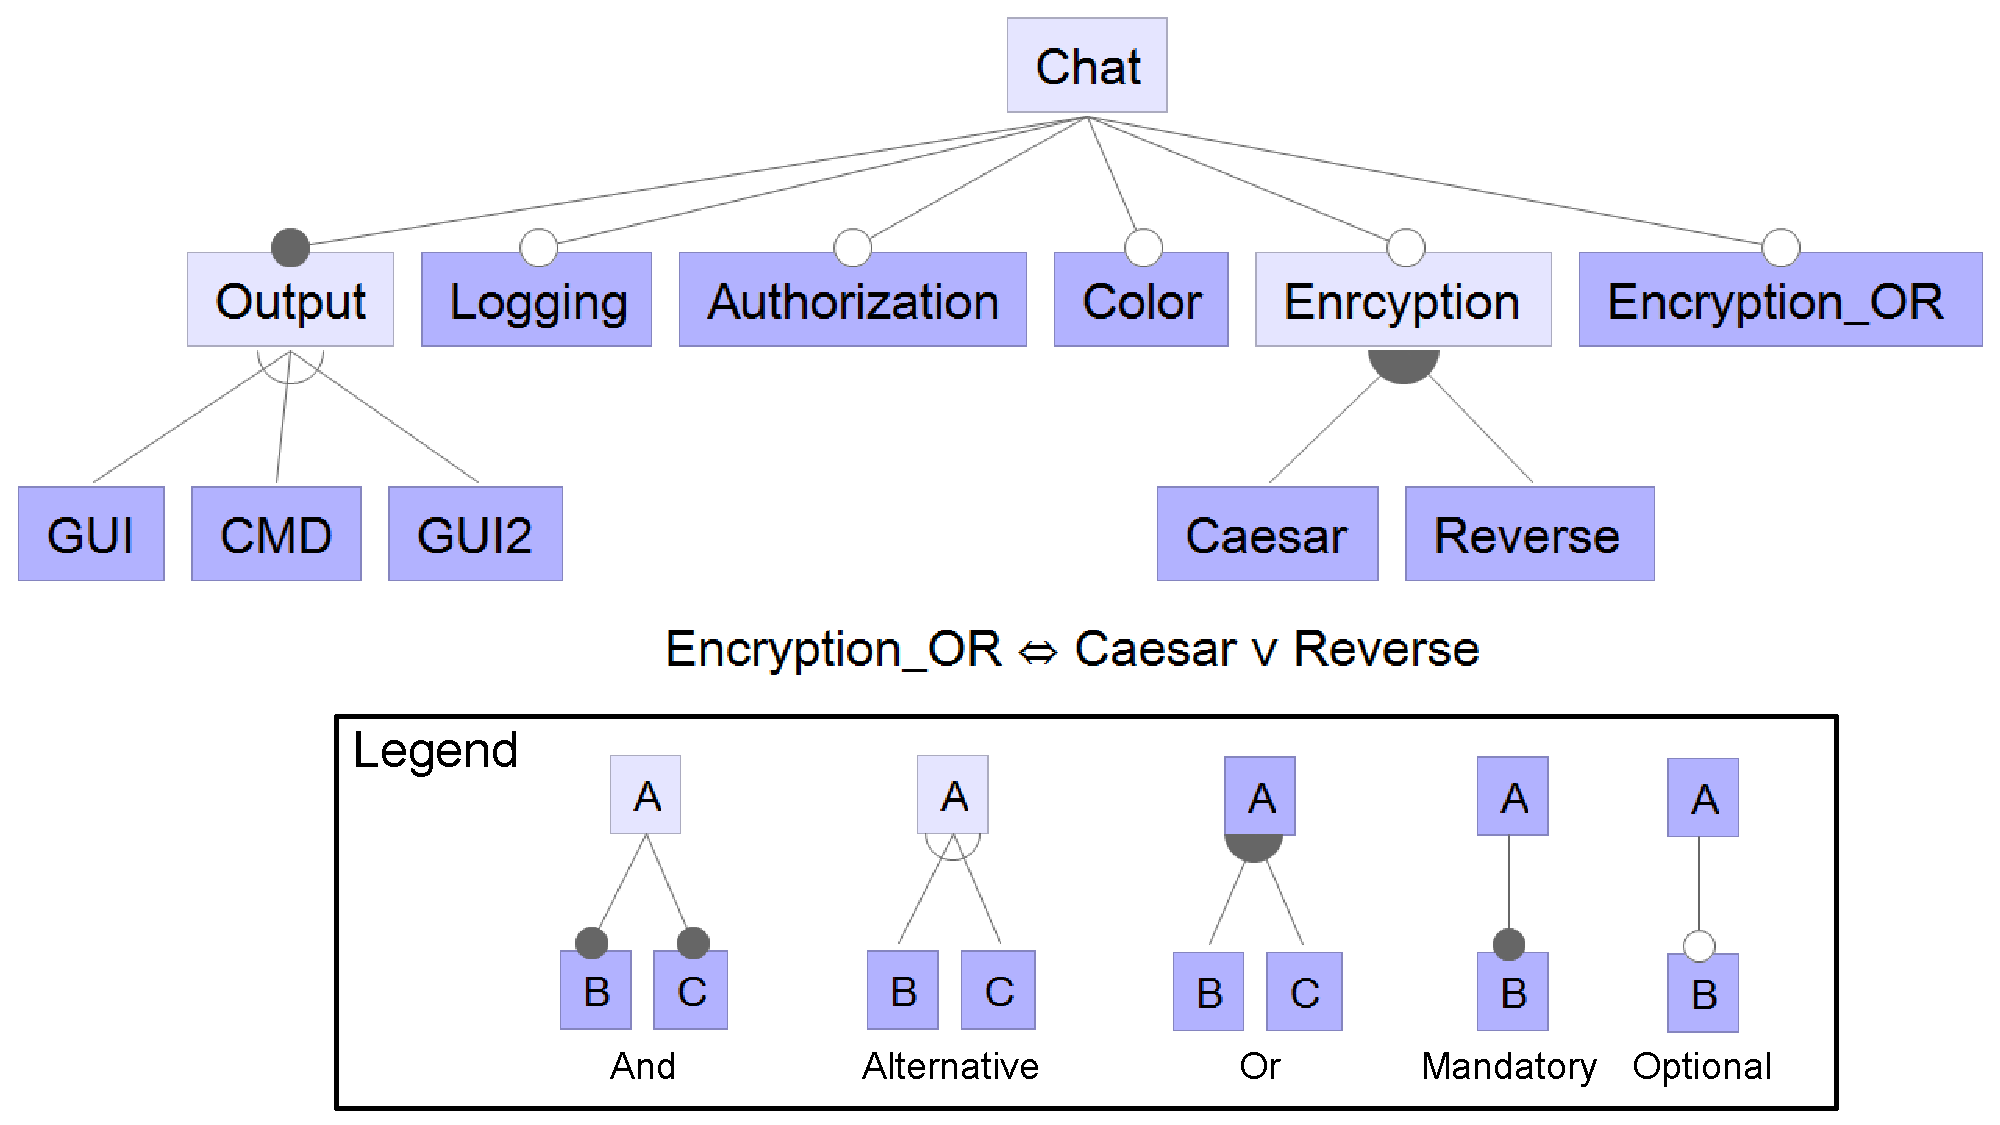
\epsfig{file=image/fm.bmp, width=8.5cm}
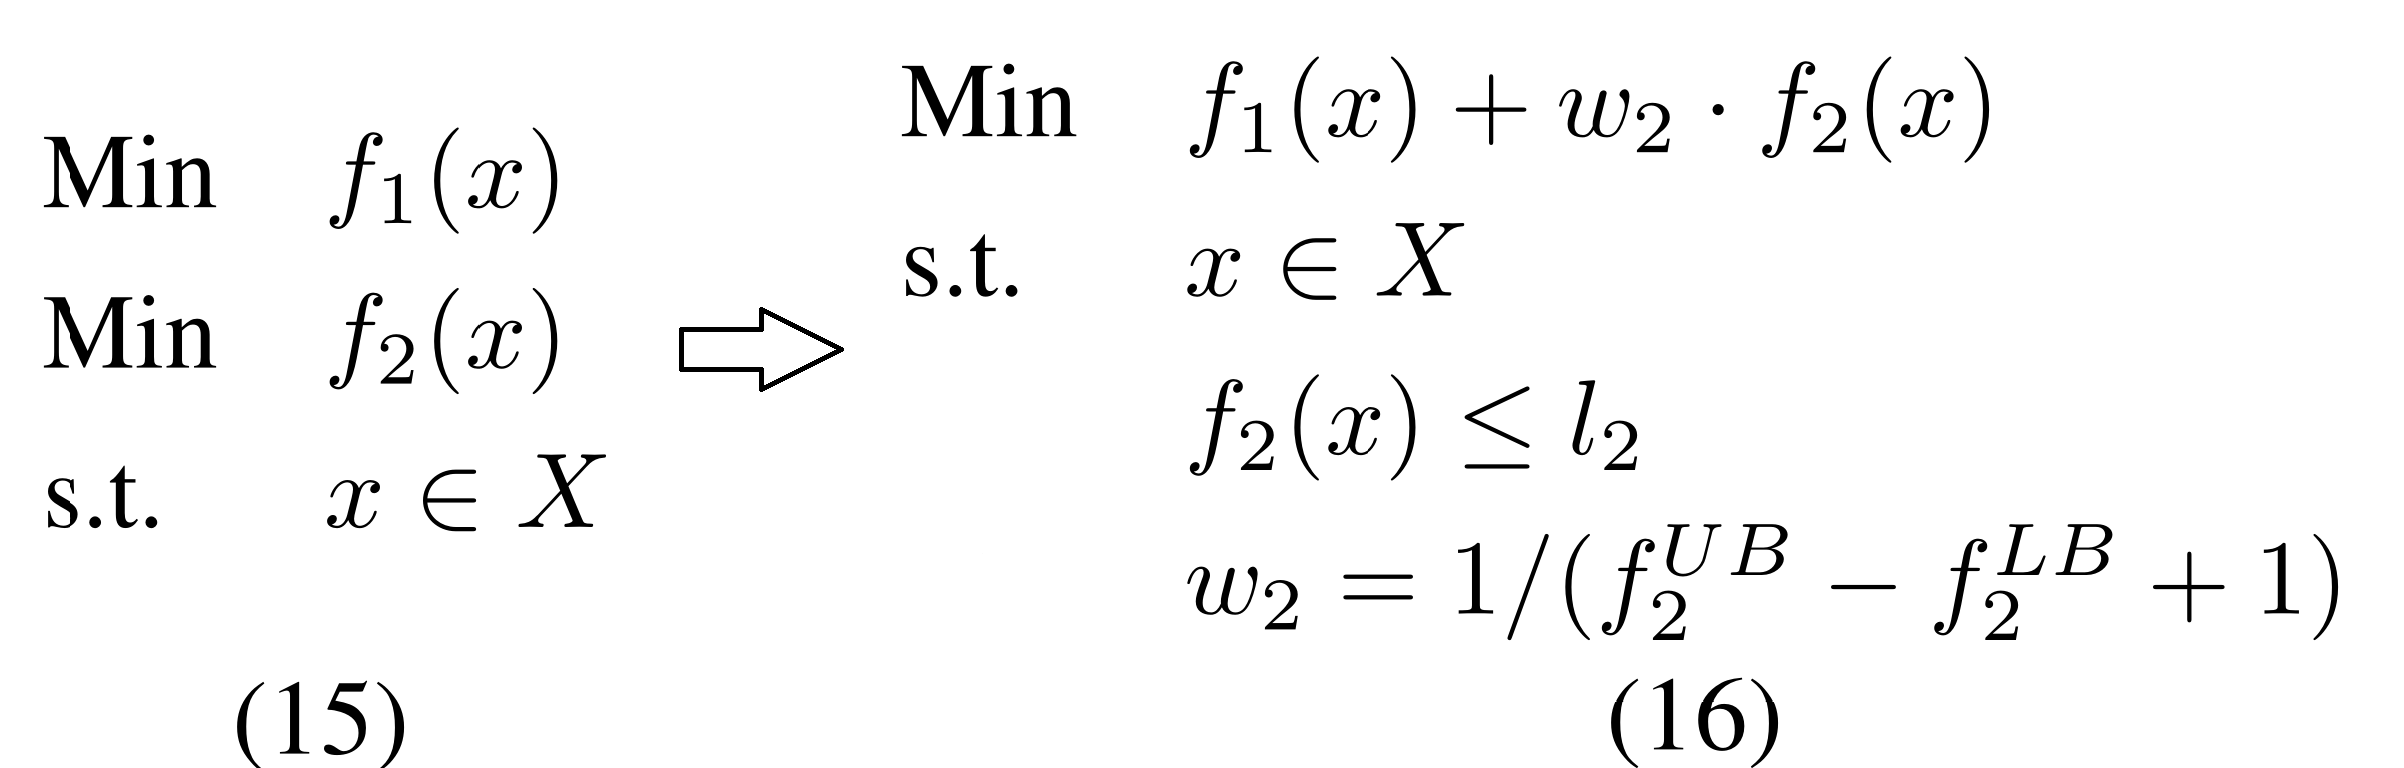
\includegraphics[width=7.8cm]{image/CWMOIP.png}
\vspace{-3.5mm}
\caption{An example of applying CWMOIP for a $bi$-objective problem}
\label{fig:cwmoip_exam}
\end{figure}


\noindent\textbf{Example for (2).}  Fig.~\ref{fig:cwmoip_exam} shows an example for objective-reduction. Solving the $bi$-objective problem in formula (15)  is reduced to solving the 1-objective problem in formula (16) by \rev{$l_2$} times. It is named "constraint weighted" because of the weight $w_2$ and the constraint $ f_2(x) \le l_2$. %on the original objective $ f_2(x)$.
 Variable $l_2$ iterates from the lower bound $f^{LB}_2$ to the upper bound $f^{UB}_2$ of $ f_2(x)$. %Here, $f^{LB}_2$ (or $f^{UB}_2$) denotes the lower (or upper) bound  of $ f_2(x)$.}
%Interested readers can refer to \cite{DBLP:journals/eor/OzlenA09} for the details of the proof.



In Algorithm \ref{alg:cwmoip}, we show the general steps of finding all non-dominant solutions for any given $k$-objective BIP problem~\cite{DBLP:journals/eor/OzlenA09} (not limited to the model of our problem). The initial invocation of Algorithm \ref{alg:cwmoip} is calling $CWMOIP(k,f^{UB}_k,X)$, and then $CWMOIP(k-1,l_k,X)$ at line \ref{algo:cwmoip:f4}, recursively, until calling $CWMOIP(1,l_2,X)$. %We explain the important steps in Algorithm 2.
Initially, lines \ref{algo:cwmoip:i2} to \ref{algo:cwmoip:i4} calculate the true upper and lower bounds of the $2$-nd objective to the $k$-th, subject to the constraint set $X$ (In practice, this can be done once and results are cached for reuse). Then $w_k$ is calculated for the $k$-th objective at line \ref{algo:cwmoip:i5}. In the loop at line \ref{algo:cwmoip:f1}, the $k$-objective problem is reduced to a new \emph{(k-1)}-objective problem (line \ref{algo:cwmoip:f4}), which has the new suffix $w_k\cdot f_k(\vec x)$ for the objective function (line \ref{algo:cwmoip:f2}) and the new constraint $f_k(\vec x) \le l_k$ for the constraint set $X$ (line \ref{algo:cwmoip:f3}). If no results are found (lines \ref{algo:cwmoip:f5}-\ref{algo:cwmoip:if2}), the recursion process stops. If found, the constraint $l_k$ is tightened to the value just smaller than the largest value of  $f_k(\vec x)$ for $\vec x \in ME$. Last, BIP solving function is called when only one objective ($k=1$) is left at line \ref{algo:cwmoip:i6} to \ref{algo:cwmoip:i6:if1}.

According to \cite{DBLP:journals/eor/OzlenA09}, the maximum number of recursion is $\frac{|E|(|E|+1)...(|E|+k-2)}{2\cdot 3 \cdot ... \cdot(k-1)}$.
Note that in our example, $\mathcal{F}_1(\vec x)$ is not needed as it is always   $0$ for BIP. Thus, it is a 4-objective ($\mathcal{F}_2(\vec x)$ to $\mathcal{F}_5(\vec x)$) BIP problem. $CWMOIP()$ will reduce it to constrain-weighted 3-objective ($\mathcal{F}_2(\vec x)$ to $\mathcal{F}_4(\vec x)$); iteratively, until to a constrain-weighted 1-objective ($\mathcal{F}_2(\vec x)$) problem.
%\begin{equation}\label{formula:singLP}
%%%\begin{array}{rrclcl}
%%%\displaystyle \min_{x} & \multicolumn{3}{l}{c^T x} \\
%%%\textrm{s.t.} & A x & \geq & b \\
%%%%&\displaystyle \sum_{i=0}^{n} x_i & = & 1 \\
%%%& x_i & \in & \{0,1\} & & \forall i \in \{1...n\} \\
%\begin{array}{ll@{}r@{}r@{}l}
%     \text{Min} & f_1(x) \\[\jot]
%     \text{Min} & f_2(x) \\[\jot]
%     \text{s.t.}& x \in X\\[\jot]
%  \end{array}
%\vspace{-3mm}
%%%\end{array}
%\end{equation}
%
%%\subsection{Preliminary Evaluation Results}
%\begin{equation}\label{formula:singLP}
%%%\begin{array}{rrclcl}
%%%\displaystyle \min_{x} & \multicolumn{3}{l}{c^T x} \\
%%%\textrm{s.t.} & A x & \geq & b \\
%%%%&\displaystyle \sum_{i=0}^{n} x_i & = & 1 \\
%%%& x_i & \in & \{0,1\} & & \forall i \in \{1...n\} \\
%\begin{array}{ll@{}r@{}r@{}l}
%     \text{Min} & f_1(x) + w_2 \cdot f_2(x)\\[\jot]
%     \text{s.t.} &  x \in X \\[\jot]
%     \text{s.t.}& f_2(x) \le l_2\\[\jot]
%     \text{s.t.}& w_2 = 1 / (f^{UB}_2-f^{LB}_2+1) \\[\jot]
%  \end{array}
%\vspace{-3mm}
%%%\end{array}
%\end{equation}
%

\section{Representation Generation Approach --- \ourSol}\label{sec:solution}
%In literature, there are three main approaches for solving multi-objective optimization problems: exact methods, meta-heuristic methods \cite{deb2001} and approximation methods \cite{ruzika2005approximation}. Exact methods aim to generate the entire Pareto front. {\color{red} i suggest to remove this paragraph, it seems to be not quite relevant here}
\vspace{-1mm}
The optimal feature selection problem is essentially a combinatorial problem. %Due to the non-convex nature of such problems, it is typically infeasible to obtain a closed-form representation of the Pareto front via CWMOIP \rev{[??]}. Further,
The number of non-dominant solutions grows exponentially along the number of features and objectives. Given its NP-hardness, it is neither practical nor necessary to find the entire true Pareto front \cite{koksalan2009multiobjective}. %as $\epsilon$-constraint approach and CWMOIP do.
Instead, obtaining a set of solutions that evenly distributed over the true Pareto front is representative, pragmatic and computationally referrable.

%\subsection{\ourSol~Method}\label{sec:solution:nc}
The normal constraint (NC) method \cite{normalCons} is an effective method in the literature that guarantees generating evenly distributed solutions over the entire Pareto front. The main idea of NC method is to use the \emph{utopia plane} to approximate the true Pareto front such that a set of evenly distributed reference points on \emph{utopia plane} would result to a set of evenly distributed solutions on Pareto front, after the projection along the normal vector of \emph{utopia plane}. Here, \emph{utopia plane} refers to the hyper plane determined by all the anchor points, each of which individually optimizes a single objective (e.g. $y_{1}^*$ for $y_1$-axis and $y_{2}^*$ for $y_2$-axis in Fig~\ref{fig:uhre}.a). However, the original NC method was developed on continuous solution space. In the case of IP, it can generate dominated solutions (see Fig~\ref{fig:uhre}.a) where point A is the solution generated using NC, but there exists a point B outside the shaded feasible region, dominating A. Therefore, we propose to combine the idea of \emph{utopia plane} and the $\epsilon$-constraint method such that all solutions are guaranteed to be non-dominant ones (see Fig~\ref{fig:uhre}.c).

\begin{figure}[t]
\vspace{-1mm}
\centering
%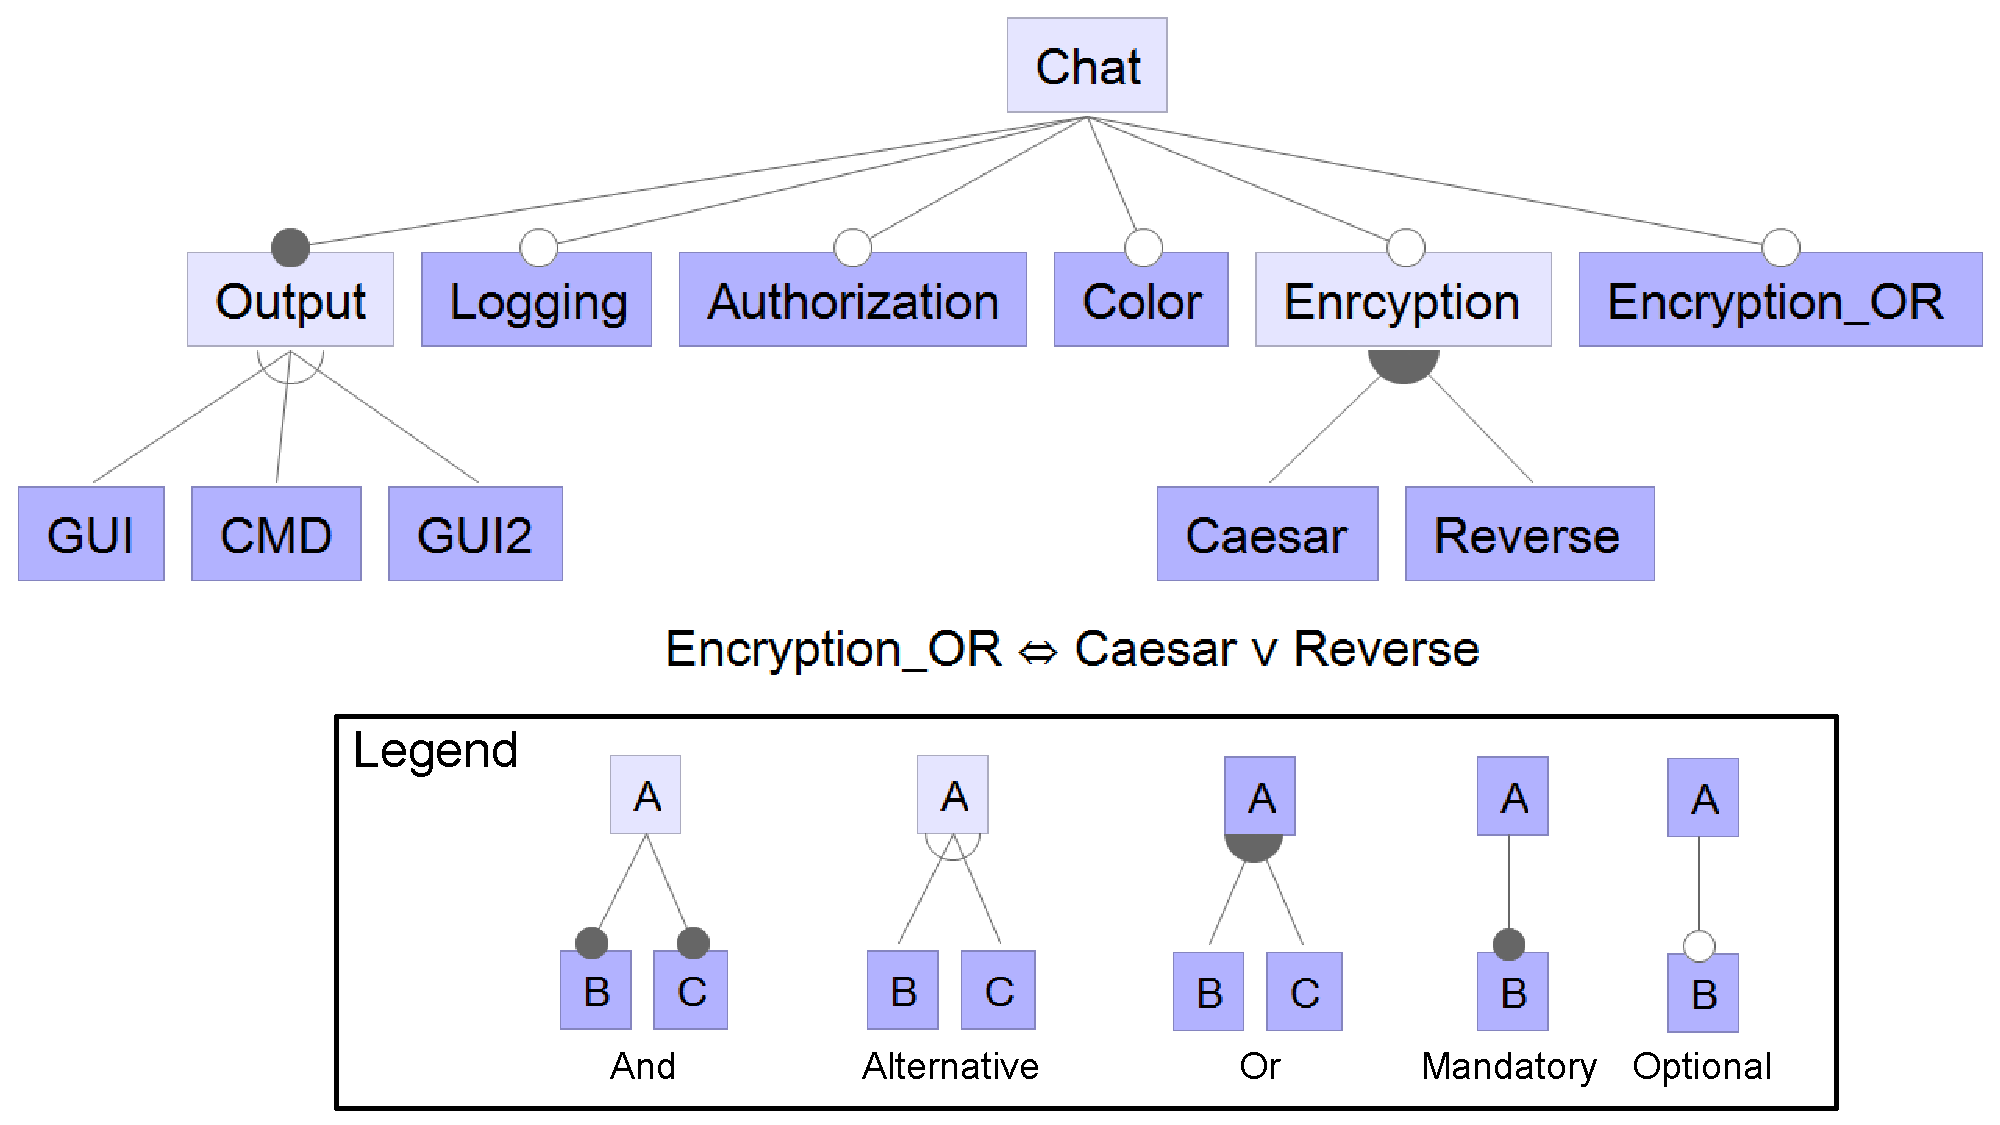
\epsfig{file=image/fm.bmp, width=8.5cm}
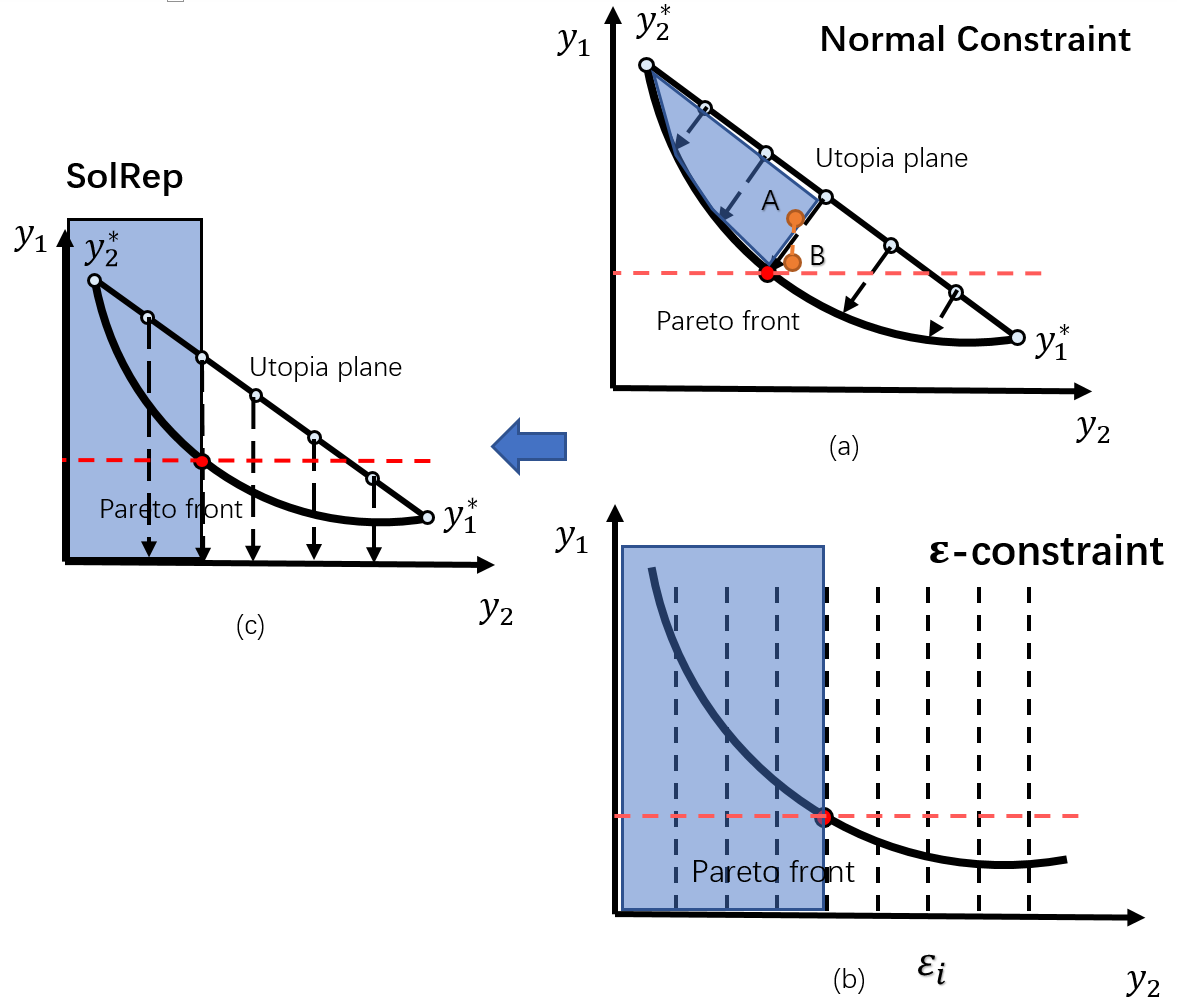
\includegraphics[width=8cm]{image/uhre.png}
\vspace{-3mm}
\caption{Two dimensional illustration of the proposed \ourSol~method}
\label{fig:uhre}
\end{figure}

Our proposed method consists of four main steps: 1) determine the utopia plane; 2) generate uniformly distributed reference points on the utopia plane; 3) for each reference point, use its $(k-1)$ coordinates to constrain the $(k-1)$ objectives; 4) optimize the $k$-th objective within the reduced solution space. Repeat steps 2) to 4) to achieve the representative Pareto front. In step 2), we resort to the hit-and-run (H\&R) method \cite{DBLP:journals/ior/Smith84} to sample the reference points.
%\rev{please insert this paper to reference list: Smith R L. Efficient Monte Carlo Procedures for Generating Points Uniformly Distributed Over Bounded Regions[J]. Operations Research, 1984, 32(6):1296-1308.}
Its principle is straightforward: let $p_{t}$ denote the current point then $p_{t+1} = p_{t} + \lambda*d$ is the next point, where $d$ is a random direction vector and $\lambda$ is the random length of the jump. As a random-walk algorithm, H\&R is proven to generate uniformly distributed points inside any polyhedron after a sufficient number of runs \cite{DBLP:journals/ior/Smith84}.

Note that an obvious alternative is to equally divide the Pareto front along each objective direction and then traverse each grid. However, it might not evenly cut the Pareto front and the computational efforts grow exponentially along the number of objectives.

\begin{algorithm}[t]                  % enter the algorithm environment
\caption{Function \small{\emph{SolRep()}} for $k$-objective IP}\label{alg:nchr}
\small
    %\KwIn{$M$: the feature model of the given system} %$maxIter$: the maximum number of iterations of the generation process
    \KwIn{$k$: the number of objectives, $N$: number of reference points, $X$: the set of linear constraints, $f_{i}$ coefficient vector of the $i$-th objective function}
    %\KwIn{$userInfor$: the contextual information of user device} %$maxIter$: the maximum number of iterations of the generation process
    \KwOut{$E$: the set of representative non-dominant solutions}
    %\KwOut{$returnedSol$: a solution returned to guide malware generation }
    \For{$ i = 1; i < k; i=i+1 $}{ \label{algo:nchr:i1}
    $y_{anch,i}= bintprog(X,f_{i})$\; \label{algo:nchr:i2}
    }
    $ ...$//determine the vertexes of utopia plane\; \label{algo:nchr:i3}
    $p_{0} = randPoint(y_{anch})$\; \label{algo:nchr:i4}
    $ ...$//generate a initial reference point $p_0$ on utopia plane\; \label{algo:nchr:i5}
    $P~\leftarrow~\emptyset, P = P \cup \{p_{0}\}$\; \label{algo:nchr:i6}
    \For{$ i = 1; i < N; i=i+1 $}{ \label{algo:nchr:i7}
    $d = randDirect(y_{anch})$\; \label{algo:nchr:i8}
    $\lambda_{range} = linprog(X,d,p_{0})$\; \label{algo:nchr:i9}
    $\lambda = unifrnd(\lambda_{range})$\; \label{algo:nchr:i10}
    $p_{0} = p_{0}+\lambda * d $\; \label{algo:nchr:i11}
    $P = P \cup \{p_{0}\}$\; \label{algo:nchr:i12}
    }
    $ ...$//find the other N-1 reference points\; \label{algo:nchr:i13}
    $E~\leftarrow~\emptyset$\; \label{algo:nchr:i14}
    \For{$ i = 1; i \le N; i=i+1 $}{ \label{algo:nchr:i15}
    $E = E \cup bintprog(X,f_{k},P_{i})$ \label{algo:nchr:i16}
    }
    \KwRet $E$;\label{algo:cwmoip:rt}
      %  $allMal\leftarrow allMal \cup newGeneration$\;\label{algo:cmb:23}

\end{algorithm}

The proposed \ourSol~method is presented in Algorithm \ref{alg:nchr}, which has the time complexity of $O(n)$ (consider $bintprog(X,f_{i})$ has $O(1)$, as a time limit is set for IP solving). The function $bintprog(X,f_{i})$ optimizes the $i$-th objective and returns one anchor point, $randPoint(y_{anch})$ generates a random initial reference point on utopia plane, $randDirect(y_{anch})$ returns a random direction vector, $linprog(X,d,p_{0})$ returns the upper and lower bounds of the jumping length $\lambda$, $unifrnd(\lambda_{range})$ returns one random length within the bounds, $bintprog(X,f_{k},P_{i})$ optimizes the $k$-th objective with the constraints incurred by the reference point $P_{i}$.
%As mentioned in Introduction Section, the drawbacks of meta-heuristic methods are: 1) non-guarantee of achieving the true Pareto optimal solutions; 2) the diversity of the obtained solutions over the entire solution space might not be guaranteed also.

%The normal boundary intersection (NBI) method \cite{das1998normal}. It generates non-Pareto and locally Pareto solutions \cite{messac2004normal}.
%The normal constraint (NC) method \cite{messac2004normal} guarantees the evenly distributed solutions over the entire Pareto front. In this method, the MOO problem is converted into one single objective optimization problem which is solved iteratively subject to a properly designed set of constraints. Different from the normal boundary intersection method, which requires the solutions being on the normal line.

%A comparative study by Messac et al. \cite{messac2003normalized} shows that NC performs favorably contrasting against NBI and physical programming. It is more computationally stable and is less likely trap to non-Pareto or locally Pareto solutions.


%\newcommand{\tool}{NCGOP~}

\section{Evaluation}\label{sec:application}
\noindent\textbf{Implementation.} To conduct a fair comparison between the MOIP methods and other MOEAs, we use the existing EAs from the open source tool of IBED \cite{DBLP:journals/asc/XueZT0CC016}. We implement these MOIP methods in the \textsc{IBED} framework. These MOIP methods are mainly implemented in Java, only the IP solving method uses the APIs of \textsc{Cplex}~\cite{CPLEX}. Our tool and experimental data are published at~\cite{ourtool}.%\footnote{CPLEX: The industrial solution for IP. \url{https://www-01.ibm.com/software/commerce/optimization/cplex-optimizer/}}. Our tool and experimental data are published at [].\footnote{IBED's tool \cite{DBLP:journals/asc/XueZT0CC016} is open-source. It extends the implementation of feedback-directed IBEA \cite{DBLP:conf/issta/TanXCSLD15} that is based on the open-source library \textsc{jMetal}.}

\noindent\textbf{Research Questions.} For \naiveSol~and CWMOIP that search for all non-dominant solutions, we answer the RQ1-RQ2.
For \ourSol~that aims to efficiently find evenly-distributed non-dominant solutions, we compare it with the state-of-the-art MOEAs (i.e., IBED and IBEA) and answer the RQ3-RQ5:
%We conducted the experiments to evaluate the above approaches from different aspects.
\vspace{-1mm}
\begin{enumerate}[label=\textbf{RQ\arabic*.},itemindent=*,itemsep=0.1mm]
\item On small systems, can  the \naiveSol~and CWMOIP guarantee the \emph{completeness} of non-dominant solutions?
\item On small systems, what is the \emph{performance} of the \naiveSol~and CWMOIP?

\item On medium-to-large systems, can \ourSol~find \emph{abundant} and \emph{non-dominant} solutions?

\item On medium-to-large systems, can \ourSol~find \emph{evenly-distributed} non-dominant solutions ?

\item On large industrial systems, is  \ourSol~\emph{scalable}?

\end{enumerate}
\subsection{Setup}\label{subsection:qualityindicator}~\label{ssec:setup}
\vspace{-3mm}
\subsubsection{Baseline Tools}\label{subsecc:implementationsetup}
%We have implemented our approach based on \textsc{jMetal}~\cite{DBLP:journals/aes/DurilloN11}, which is a Java-based open source framework that supports multi-objective optimization with EAs.
Sayyad \emph{et.al} \cite{DBLP:conf/icse/SayyadMA13,conf/cmsbse/SayyadMA13} reported that IBEA implemented in \textsc{jMetal} shows best results for the optimal feature selection. %Later, Tan \emph{et.al} \cite{DBLP:conf/issta/TanXCSLD15} also proposed the feedback-directed mechanism to improve existing MOEAs. In these studies, IBEA is reported as the best MOEA for this problem.
Recently, according to \cite{DBLP:journals/asc/XueZT0CC016}, on most systems (except $eCos$), IBED finds more non-dominant solutions than IBEA in similar time.  IBEA and IBED represent the-state-of-art approaches and they are publicly available. Hence, we choose them as the baseline tools for comparison.

%\textbf{IBEA}: Indicator-Based Evolutionary Algorithm ~\cite{DBLP:conf/ppsn/ZitzlerK04}.

%\begin{enumerate}[itemindent=*,itemsep=0.1mm]
%   \item \textbf{our approach}: our Indicator-Based Differential Evolutionary
%   \item \textbf{IBEA}: Indicator-Based Evolutionary Algorithm ~\cite{DBLP:conf/ppsn/ZitzlerK04}
%  \item \textbf{NSGA-II}: Nondominated Sorting Genetic Algorithm ~\cite{DBLP:journals/tec/BradstreetWB08}
%  \item \textbf{ssNSGA-II}: Steady-state NSGA-II ~\cite{coello2004applications}
%  \item \textbf{MOCell}: A Cellular Genetic Algorithm for Multi-objective Optimization~\cite{miettinen1999nonlinear}
%\end{enumerate}
%A brief overview of these EAs are provided in~\mtable{table:EAOverview}.

% Table generated by Excel2LaTeX from sheet 'Sheet1'
% Table generated by Excel2LaTeX from sheet 'Sheet1'

\subsubsection{Baseline Tools Configurations}
We adopt the version of IBEA and IBED that produce the best results according to \cite{DBLP:conf/issta/TanXCSLD15}\cite{DBLP:journals/asc/XueZT0CC016} --- actually the same enhancement for them, namely \textbf{IBED $F+P$} and \textbf{IBEA $F+P$}. Here $F+P$ refers to the configuration that enables feedback-directed mechanism \cite{DBLP:conf/issta/TanXCSLD15} and preprocessing for core feature encoding \cite{DBLP:journals/tosem/HieronsLLSZ16}.
%\begin{enumerate}[label=\alph*),itemsep=0.1mm]
 % \item \textbf{IBEA $F+P$}: the IBEA version that enable feedback-directed mechanism \cite{DBLP:conf/issta/TanXCSLD15} and pre.
  %  \item \textbf{IBED $F+P$}: the IBED version that enable feedback-directed mechanism and core
%  \item \textbf{U+P}: The unguided version of EA with preprocessing  (\msection{ssec:preprocess}) applied before the execution of the unguided EA. We have demonstrated that, our method has found more prunable features than the preprocessing method of~\cite{DBLP:dblp_conf/kbse/SayyadIMA13} in~\msection{subsecc:featuremodelsetup}; therefore, U+P can be seen as an improved version of~\cite{DBLP:dblp_conf/kbse/SayyadIMA13} with smaller search space.
%  \item \textbf{U}: The unguided version of EA without preprocessing, which is used by~\cite{DBLP:conf/icse/SayyadMA13,conf/cmsbse/SayyadMA13}.

   %this is essentially the version that has been used in~\cite{DBLP:conf/icse/SayyadMA13}, which is the current state-of-the-art method to the knowledge of the authors.
%\end{enumerate}


%\begin{table}[t]
%  \centering
%  \vspace{-2mm}
%    \caption{Feature Models}
%   \scalebox{0.85}{
%   % Table generated by Excel2LaTeX from sheet 'Sheet2'
%\begin{tabular}{|>{\centering\arraybackslash}m{0.5cm}|>{\centering\arraybackslash}m{1.2cm}|>{\centering\arraybackslash}m{0.7cm}|>{\centering\arraybackslash}m{0.95cm}|>{\centering\arraybackslash}m{0.6cm}|>{\centering\arraybackslash}m{0.6cm}|>{\centering\arraybackslash}m{0.95cm}|}
%\hline
%\multicolumn{1}{|c|}{\textbf{Repo.}} & \textbf{Sys.} & \textbf{Fea.} & \textbf{Cons.} & \textbf{$F_p$} & \textbf{$F_p'$} & \multicolumn{1}{c|}{\textbf{Ref.}} \bigstrut\\
%\hline
%    --  & JCS   & 12    & 13    &    2   &    --  & -- \bigstrut\\
%\hline
%\multicolumn{1}{|c|}{\multirow{2}[4]{*}{SPLOT}} & Web Portal & 43    & 36    &    4   &    --   & \cite{DBLP:conf/sac/MendoncaBC08}
%  \bigstrut\\
%\cline{2-7}\multicolumn{1}{|c|}{} & E-Shop & 290   & 186   &   28    &   --    & \cite{DBLP:conf/wcre/XueXJ10} \bigstrut\\
%\hline
%\multicolumn{1}{|c|}{\multirow{4}[10]{*}{LVAT}} & eCos  & 1244  & 3146  &  54     &  19     & \cite{DBLP:conf/icse/SheLBWC11,DBLP:conf/wcre/XueXJ10} \bigstrut\\
%%\cline{2-7}\multicolumn{1}{|c|}{} & FreeBSD & 1396  & 62183 &    41   &    3  & \cite{DBLP:conf/icse/SheLBWC11,thTechnireport10} \bigstrut\\
%%\cline{2-7}\multicolumn{1}{|c|}{} & Fiasco & 1638  & 5228  &   1013    &   995   &\cite{Berger12variabilitymodeling}  \bigstrut\\
%\cline{2-7}\multicolumn{1}{|c|}{} & uClinux & 1850  & 2468  &   1244    &  1244    & \cite{Berger12variabilitymodeling} \bigstrut\\
%\cline{2-7}\multicolumn{1}{|c|}{} & Linux X86 & 6888  & 343944 &   156    &   94    & \cite{DBLP:conf/icse/SheLBWC11} \bigstrut\\ %,thTechnireport10
%\hline
%\end{tabular}%
%     }
%
%\vspace{-4mm}
%  \label{table:feaModel}%
%\end{table}%

% Table generated by Excel2LaTeX from sheet 'Sheet4'
% Table generated by Excel2LaTeX from sheet 'Sheet4'
\begin{table}[bp]
 
  \centering
  \scriptsize
    \caption{Feature Models used in experiments}
    \begin{tabular}{|c|c|c|c|c|}
    \hline
    \textbf{Repo.} & \textbf{Sys.} & \textbf{Fea.} & \textbf{Cons.} & \multicolumn{1}{c|}{\textbf{Ref.}} \bigstrut\\
    \hline
    \multirow{3}[6]{*}{SPLOT} & JCS   & 12    & 12    &  \cite{DBLP:conf/issta/TanXCSLD15} \bigstrut   \\
\cline{2-5}          & Web Portal & 43    & 36    &  \cite{DBLP:conf/sac/MendoncaBC08} \bigstrut\\
\cline{2-5}          & E-Shop & 290   & 186   &  \cite{DBLP:conf/wcre/XueXJ10} \bigstrut\\
    \hline
    \multirow{3}[6]{*}{LVAT} & eCos  & 1244  & 3146  &  \cite{DBLP:conf/icse/SheLBWC11,DBLP:conf/wcre/XueXJ10} \bigstrut\\
\cline{2-5}          & uClinux & 1850  & 2468  &  \cite{Berger12variabilitymodeling} \bigstrut\\
\cline{2-5}          & LinuxX86 & 6888  & 343944 & \cite{DBLP:conf/icse/SheLBWC11}  \bigstrut\\
    \hline
    \end{tabular}%
 
  \label{table:feaModel}%
\end{table}%



% Table generated by Excel2LaTeX from sheet 'Sheet3'

\begin{table*}[t]
  \centering
  \scriptsize
  \vspace{-3mm}
  \caption{Non-dominant solutions found by $\epsilon$-constraint (\textbf{A})  and CWMOIP  (\textbf{B})   on two small models, with 4 attribute sets for each model}
    \begin{tabular}{|c|c|c|c|c|c|c|c|c|c|c|c|c|c|c|}
   \Xhline{2\arrayrulewidth}
    System & A \%Corr & B \%Corr & A Time(s) & B Time(s) &A HV & B HV & A SP & B SP & $|A|$ & $|B|$ & $|A \cap B|$ & \textbf{$|N_A \cup N_B|$} & \textbf{$|N^{U}_A|$} & \textbf{$|N^{U}_B|$} \bigstrut\\
   \Xhline{2\arrayrulewidth}
    JCS 1 & 100   & 100   & 5.11  & 1.66  & 0.29  & 0.29  & 0.69  & 0.69  & 39    & 39    & 39    & 39    & 0     & 0 \bigstrut\\
    \hline
    JCS 2 & 100   & 100   & 6.84  & 0.67  & 0.27  & 0.27  & 0.39  & 0.39  & 9     & 9     & 9     & 9     & 0     & 0 \bigstrut\\
    \hline
    JCS 3 & 100   & 100   & 3.54  & 0.96  & 0.29  & 0.29  & 0.43  & 0.43  & 22    & 22    & 22    & 22    & 0     & 0 \bigstrut\\
    \hline
    JCS 4 & 100   & 100   & 7.92  & 1.97  & 0.25  & 0.25  & 0.56  & 0.56  & 31    & 31    & 31    & 31    & 0     & 0 \bigstrut\\
    \hline
    Web Portal 1 & 100   & 100   & 570.68  & 212.22  & 0.34  & 0.34  & 0.87  & 0.87  & 451   & 451   & 451   & 451   & 0     & 0 \bigstrut\\
    \hline
    Web Portal 2 & 100   & 100   & 692.88  & 256.38  & 0.31  & 0.31  & 0.98  & 0.98  & 768   & 768   & 768   & 768   & 0     & 0 \bigstrut\\
    \hline
    Web Portal 3 & 100   & 100   & 696.83  & 237.75  & 0.32  & 0.32  & 0.92  & 0.92  & 859   & 859   & 859   & 859   & 0     & 0 \bigstrut\\
    \hline
    Web Portal 4 & 100   & 100   & 564.82  & 163.97  & 0.33  & 0.33  & 0.96  & 0.96  & 713   & 713   & 713   & 713   & 0     & 0 \bigstrut\\
    \hline
    \end{tabular}%
  \label{tab:naiveVScwmoip}%
\vspace{-3mm}
\end{table*}%

\subsubsection{Parameter Settings}
 %For $U$, the same as~\cite{conf/cmsbse/SayyadMA13}, single-point crossover and bit-flip mutation are used as crossover and mutation operators, with crossover and mutation probabilities set to 0.1 and 0.01 respectively. These operators and probabilities also apply to $U+P$.
 For the $F+P$ version of EAs, %the feedback-directed  crossover  and feedback-directed mutation operators are used.
according to \cite{DBLP:conf/issta/TanXCSLD15}\cite{DBLP:journals/asc/XueZT0CC016},  the best setting of error mutation probability, mutation probability, and crossover probability are  1.0, 0.0000001, and 0.1 respectively. %Note in \mtable{table:lvat}, configuration $\mathit{F'+P}$ is the same as $\mathit{F+P}$, with the exception that the mutation probability $\mathit{P_{mut}}$ is set to 0.01.
%We run two settings for crossover probability $P_{cross}$, and mutation probability $P_{mut}$, which are $P_1=\{P_{Cross}=0.9, P_{mut}=0.05\}$ and $P_2=\{P_{Cross}=0.1, P_{mut}=0.01\}$. Configuration $U$ with parameter setting $P_1$ is used in ~\cite{DBLP:conf/icse/SayyadMA13}, and configuration $U$ with  parameter setting $P_2$ is used in ~\cite{conf/cmsbse/SayyadMA13}. These are the state-of-the-art methods for the optimal feature selection, to the knowledge of the authors.
For SPLOT systems in Table \ref{table:feaModel}, 25000 evaluations are used  for IBEA and IBED. For larger LVAT systems, 100000 evaluations are used for both EAs. For any model, we generate 10 sets of attributes. For each set, we run each EA repeatedly for 30 times and use their union to compare with \ourSol. Besides, the medium execution (the medium values of metrics) is compared with \ourSol~using 50 reference points. %The evaluation results for SPLOT and LVAT are reported in~\mtable{table:splot} and~\mtable{table:lvat}, respectively.
All other parameter settings for EAs are default settings of \textsc{jMetal} (e.g., population size is set to 100) are same as those used in \cite{DBLP:conf/icse/SayyadMA13}\cite{conf/cmsbse/SayyadMA13}\cite{DBLP:conf/issta/TanXCSLD15}\cite{DBLP:journals/asc/XueZT0CC016}.

In MOIP methods,  one common parameter is needed --- time limited for function $bintprog$. We set it as 0.1s for all system except for \emph{Linux X86} (10s for this system due to its huge number of constraints). The setting for reference point number in \ourSol~is 1000 for SPLOT  systems and 1500 for LVAT.


 The experiments were performed on an Intel Core I7 4710HQ CPU with 8 GB RAM, running on Windows 8.1.
%
%\paratitle{Parameters Setup} The mutation and crossover rates for rGA are set to 0.01% and 0.9%
%respectively. In addition, the population size is set to 20, the number
%of generations is set to 20.

\subsubsection{Quality Indicators}

To measure the quality of Pareto front, we adopt four indicators in this work:  percentage of correctness, hypervolume~\cite{DBLP:journals/tec/ZitzlerT991}, spread~\cite{DBLP:journals/tec/BradstreetWB08} and Pareto dominance.

%Hypervolume~\cite{DBLP:journals/tec/ZitzlerT991} is a measure measures of the volume of the dominated portion of the objective space.
% \begin{figure}[t]
%\centering
%\includegraphics[width=2.5in]{image/space}
%\caption{Hypervolume of a solution set with three solutions}
%\label{fig:hyper}
%\end{figure}

\begin{enumerate}[label=\alph*), itemsep=0.1mm]

  \item \textbf{\emph{Percentage of Correctness} (\%Cor)}:  For MOEAs, not all solutions are correct, as correctness is an objective evolving over time. Thus, for a solution set, the percentage of correct solutions inside indicates its quality.
  \item \textbf{\emph{Hypervolume (HV)}}: Hypervolume of the solution set $S$ is the volume of the region that is dominated by $S$ in the objective space. In \textsc{jMetal}, %though all objectives are minimized, the Pareto front is inverted before HV is calculated. Thus,
      the Pareto front with a higher HV is preferred.


\item \textbf{\emph{Spread (SP)}}: Spread is  used to measure the extend of spread in the obtained solutions.% and it is calculated using the following equation:
%\vspace{-1mm}
%\begin{equation}\label{eq:spread}
%\scriptsize
%Spread= \frac{d_f+d_l+\sum_{i=1}^{N-1}|d_i-\bar{d}|}{d_f+d_l+(N-1)\bar{d}}
%\end{equation}

\item \textbf{\emph{Num. of Pareto non-dominance}}: On the same set of feature attribute values, we can approximate the true Pareto front by the union of the two sets of solutions. On this Pareto front, we count the non-dominant solutions.
 %The larger the num. is, the higher quality the solutions are of. }
%      where $\mathit{N}$ is the number of points in the Pareto front, $\mathit{d_i}$ is Euclidean distances between consecutive points,  $\mathit{\bar{d}}$ is the average of $\mathit{d_i}$, $\mathit{d_f}$ and $\mathit{d_l}$ are the Euclidean distances between the extreme solutions and boundary solutions of the Pareto front respectively.
\end{enumerate}


%Other quality indicators, e.g., generational distance, inverted generational distance, epsilon and generalized speed, are used elsewhere. These indicators are not adopted in this experiment since they are used to compare the calculated Pareto front with the actual true Pareto front, which we do not have in this case.



% Table generated by Excel2LaTeX from sheet 'formated results'
\begin{table*}[t]
  \centering
   \scriptsize
   \vspace{-1mm}
  \caption{Non-dominant solutions found by CWMOIP (\textbf{A}) and  IBED $F+P$ (\textbf{B}) on two small models, with 4 attribute sets for each model}
    \begin{tabular}{|c|c|c|c|c|c|c|c|c|c|c|c|c|c|c|}
  \Xhline{2\arrayrulewidth}
    System & A \%Corr & B \%Corr & A Time(s) & B Time(s) &A HV & B HV & A SP & B SP & $|A|$ & $|B|$ & $|A \cap B|$ & \textbf{$|N_A \cup N_B|$} & \textbf{$|N^{U}_A|$} & \textbf{$|N^{U}_B|$} \bigstrut\\
   \Xhline{2\arrayrulewidth}
    JCS 1 & 100   & 92.37  & 1.66  & 150.66  & 0.29  & 0.28  & 0.69  & 0.28  & 39    & 19    & 19    & 39    & 20    & 0 \bigstrut\\
    \hline
    JCS 2 & 100   & 91.72  & 0.67  & 131.19  & 0.27  & 0.27  & 0.39  & 0.39  & 9     & 9     & 9     & 9     & 0     & 0 \bigstrut\\
    \hline
    JCS 3 & 100   & 85.80  & 0.96  & 135.38  & 0.29  & 0.28  & 0.43  & 0.31  & 22    & 17    & 17    & 22    & 5     & 0 \bigstrut\\
    \hline
    JCS 4 & 100   & 84.77  & 1.97  & 135.20  & 0.25  & 0.24  & 0.56  & 0.54  & 31    & 20    & 20    & 31    & 11    & 0 \bigstrut\\
    \hline
    Web Portal 1 & 100   & 98.00  & 212.22  & 162.80  & 0.34  & 0.33  & 0.87  & 0.45  & 451   & 232   & 97    & 451   & 354   & 0 \bigstrut\\
    \hline
    Web Portal 2 & 100   & 98.73  & 256.38  & 166.67  & 0.31  & 0.30  & 0.98  & 0.63  & 768   & 277   & 116   & 768   & 652   & 0 \bigstrut\\
    \hline
    Web Portal 3 & 100   & 99.63  & 237.75  & 156.52  & 0.32  & 0.31  & 0.92  & 0.66  & 859   & 386   & 184   & 859   & 675   & 0 \bigstrut\\
    \hline
    Web Portal 4 & 100   & 96.93  & 163.97  & 163.69  & 0.33  & 0.32  & 0.96  & 0.73  & 713   & 327   & 167   & 713   & 546   & 0 \bigstrut\\
    \hline
    \end{tabular}%
  \label{tab:cwmoipVSibed}%
\vspace{-3mm}
\end{table*}%


\subsection{Evaluation Systems}\label{sec:cases}

\subsubsection{System Selection}\label{subsecc:featuremodelsetup}

Feature models of different systems are used in experiments. Table \ref{table:feaModel} shows  repository name (\emph{Repo.}),  the model's system name (\emph{Sys.}), number of features (\emph{Fea.}),  number of constraints (\emph{Cons.}), and relevant literatures (\emph{Ref.}).


Three models are from SPLOT, a repository used by many researchers as a benchmark \cite{DBLP:conf/oopsla/MendoncaBC091}. $\JCS$ model is the running example of the paper. %Two feature models \emph{Web Portal} and \emph{E-Shop} are from SPLOT respository~, which is a repository used by many researchers as a benchmark.
\emph{Web Portal} model captures the configurations of Web portal product line, and \emph{E-Shop} model %, as one of the largest feature models in SPLOT,
captures a B2C system with fixed priced products. %These two models are chosen to facilitate the comparison with~\cite{DBLP:conf/icse/SayyadMA13}.
%To further evaluate the scalability,
Industrial systems' models from the Linux Variability Analysis Tools (LVAT) repository~\cite{LVAT} are used. %The models in LVAT were reversed-engineered from industrial systems.
%In contrast with SPLOT,
LVAT's models (e.g., \emph{Linux X86}) have  much more features and constraints.
All these models are chosen to facilitate the comparison with~\cite{DBLP:conf/icse/SayyadMA13}\cite{DBLP:conf/issta/TanXCSLD15}\cite{DBLP:journals/asc/XueZT0CC016}.

%Note that $\mathit{F_p}$ always contains the same number or more features than $\mathit{F_p'}$ -- this shows that our preprocessing method  with~\malgo{algo:filter}  has found more prunable features than~\cite{DBLP:dblp_conf/kbse/SayyadIMA13}. In~\cite{DBLP:dblp_conf/kbse/SayyadIMA13}, their preprocessing method is based on static analysis. In particular, they detect  always true disjunctions (rules) with only one feature, which means the feature is either a common feature or a dead feature. In addition, they investigate the disjunctions (rules) that include two features, if one of them is prunable in the first round, and the other one could be prunable as well. It is easy to see that our method based on SAT solving could detect all features that could be found by preprocessing method in~\cite{DBLP:dblp_conf/kbse/SayyadIMA13}, and it can be shown that $\mathit{F_p}$ is always not fewer than $\mathit{F_p'}$.

\subsubsection{Feature Attribute}

Each feature in each model has the following attributes, which are identical to attributes used in~\cite{DBLP:conf/icse/SayyadMA13}:

\begin{enumerate}[label=\textbf{\arabic*.},itemindent=*,itemsep=0.1mm]
  \item \textbf{\emph{Cost}}  $\in \grandr$, records the price incurred to include the feature. For each feature, the \emph{Cost} value is assigned with a real number that is normally distributed between 5.0 and 15.0.
  \item \textbf{\emph{Used\_Before}} $\in \{true, false\}$, records whether this feature was used before --- \emph{true}  for \lq\lq{}yes\rq\rq{} and \emph{false} for \lq\lq{}no\rq\rq. \emph{Used\_Before} values are uniformly distributed for features.
%  \item \textbf{\emph{Defects}} $\in \grandZ$, records the number of defects known in the feature. For each feature, the \emph{Defects} value is assigned with a real number that is normally distributed between 5 and 15. However, if the feature has not been used before, the \emph{Defects} value is set to 0.
  \item \textbf{\emph{Defects}} $\in \grandZ$, records the number of defects in the feature. For each feature, the \emph{Defects} value is assigned with an integer value normally distributed between 0 and 10. %However, if the feature has not been used before, the \emph{Defects} value is set to 0.
\end{enumerate}


%These three attributes provides three optimization objectives, i.e., to minimize total cost, to maximize features that have been used and to minimize the total number of known defects.

%\subsubsection{Optimization Objectives}
%We introduce the five optimization objectives that we use in the experiment in the following.
%Note that since jMetal requires minimization of the objectives; all objectives listed here are objectives to be minimized.
%\begin{enumerate}[label=\textbf{Obj\arabic*.},itemindent=*,itemsep=0.1mm]
%  \item \emph{Correctness}: minimize the number of violated constraints of the feature model.
%  \item \emph{Richness of features:} minimize the number of features that are not selected.
%  \item \emph{Cost:} minimize the total cost.
%  \item \emph{Feature used before:} minimize the number of features that have not been used before.
%  \item \emph{Defects:} minimize the number of known defects.
%\end{enumerate}
%
%We specify correctness as an objective, rather than a constraint. The reason is that this allows EA to nudge the search towards feature models that contain fewer violated constraints, which eventually lead to valid feature models that do not contain violated constraints. Furthermore, note that some objectives are conflicting, e.g., Obj2 and Obj3, because the richness of features would imply a higher cost, but at the same time the cost needs to be minimized.

\subsection{Results}\label{sec:results}
To accurately compare the quality of solutions found by two methods, we check Pareto dominance-relation and other indicators (HV, SP and time).
In Table \ref{tab:naiveVScwmoip}, \ref{tab:cwmoipVSibed}, \ref{tab:ourSolVSibed} and \ref{tab:ourSolVSibea}, we  record the  \emph{\textbf{correct}} solutions  found by the first method in  column \textbf{$|A|$}, and those by the second one in column \textbf{$|B|$}. Column \textbf{$|A  \cap  B|$}  shows  the  number  of  \textbf{\emph{correct  solutions  commonly  found}}  by both methods. After non-dominance sorting, column  $|N_A \cup  N_B|$  lists  the  number of \emph{\textbf{the union of correct non-dominant}} solutions found  by  both  methods.  We also  list  the  number  of correct \emph{\textbf{unique non-dominant}} solutions  found  only by  the first  (or the second) method  in  column  $|N^U_A|$  (or  $|N^U_B|$).
To mitigate the bias due to one-time execution of EAs,  we compare MOIP methods with them based on the union of non-dominant solutions found by 30 executions of EAs.  $|Time(s)|$ refers to the total time ---- for EAs, it is total time for 30 executions. To get $|HV|$ and $|SP|$, we approximate true Pareto front with  $|N_A \cup  N_B|$ and use that as reference points.

We first evaluate the $\epsilon$-constraint and CWMOIP that aim to find all non-dominant solutions.

\subsubsection{RQ1---Solution Set Completeness on Small Systems}\label{sec:results:rq1}
As shown in  Table \ref{tab:naiveVScwmoip}, on 4 different sets of feature attributes of each model, we can always find \textbf{$|A|$}=\textbf{$|B|$}= $|N_A \cup  N_B|$, which means they found exactly same solutions. As the completeness of the $\epsilon$-constraint and CWMOIP has been proven in \cite{e-constraint}\cite{DBLP:journals/eor/OzlenA09}, we confirm this by the experiments.
Comparing CWMOIP with IBED  in  Table \ref{tab:cwmoipVSibed}, we see \textbf{IBED cannot find all non-dominant solutions with 30 executions in most cases} (except \emph{JCS2} that  has only 9 non-dominant solutions). In most cases, IBED's results are unsatisfactory, covering averagely about $70\%$ of the true Pareto front on 4 attribute sets of \emph{JCS}, and about $20\%$ of the true Pareto front on \emph{Web Portal}. Also,  we find $|N_A \cup  N_B|= |A|$, which proves the completeness of $|A|$.
% Table generated by Excel2LaTeX from sheet 'Sheet3'
\subsubsection{RQ2---Performance on Small Systems}\label{sec:results:rq2}
In Table \ref{tab:cwmoipVSibed}, we can see that it takes averagely about 5s for \naiveSol~method and 1.5s for CWMOIP on 4 attribute sets of \emph{JCS}, and averagely about 613s for \naiveSol~method and 218s for CWMOIP on 4 attribute sets of \emph{Web Portal}.
In contrast, one medium execution of IBED (i.e., the one with the medium size of $|A|$ in 30 executions)  on \emph{JCS 1} takes about 4.5s to find $17$ correct solutions. Actually, on \emph{JCS 1}, 30 executions just brings several more solutions than 1 executions, as the search space is small and EAs can converge fast. Similarly, one medium execution of IBED on \emph{Web Portal 1} takes about 5.4s to find 35 correct solutions, while 30 executions just produce $232$ correct solutions, as  many executions also share solutions. %one execution may find duplicated solutions and

In theory, the $\epsilon$-constraint and CWMOIP both have exponential time complexity (\S\ref{sec:naiveSolutions}).
In Table \ref{tab:naiveVScwmoip} and \ref{tab:cwmoipVSibed}, experimental results confirm that --- \textbf{from 12 features (\emph{JCS}) to 43 features (\emph{Web Portal}), the time of $\epsilon$-constraint and CWMOIP increases by at least 100-fold, respectively}. We run CWMOIP on any attribute set of \emph{E-Shop} (290 features), and in 6 hours it cannot finish.

To make MOIP methods scalable and effective, we propose \ourSol~and evaluate this method in the following subsections.
% Table generated by Excel2LaTeX from sheet 'formated results'
\begin{table*}[htbp]
  \centering
    \vspace{-3mm}
  \scriptsize
   \caption{Non-dominant solutions found by \ourSol~(\textbf{A}) and  IBED $F+P$ (\textbf{B}) on SPLOT and LVAT models. On \emph{LinuxX86}, IBED uses 3 seed solutions.}
    \begin{tabular}{|c|c|c|c|c|c|c|c|c|c|c|c|c|c|c|}
  \Xhline{2\arrayrulewidth}
    System & A \%Corr & B \%Corr & A Time(s) & B Time(s) &A HV & B HV & A SP & B SP & $|A|$ & $|B|$ & $|A \cap B|$ & \textbf{$|N_A \cup N_B|$} & \textbf{$|N^{U}_A|$} & \textbf{$|N^{U}_B|$} \bigstrut\\
   \Xhline{2\arrayrulewidth}
    JCS 1  & 100   & 92.37  & 2.59  & 150.66  & 0.28  & 0.28  & 0.65  & 0.27  & 29    & 19    & 14    & 34    & 15    & 5 \bigstrut\\
    \hline
    JCS 2  & 100   & 91.72  & 2.28  & 131.19  & 0.26  & 0.27  & 0.76  & 0.39  & 4     & 9     & 4     & 9     & 0     & 5 \bigstrut\\
    \hline
    WebPortal 1 & 100   & 98.00  & 6.28  & 162.80  & 0.30  & 0.32  & 0.54  & 0.48  & 120   & 232   & 39    & 188   & 81    & 68 \bigstrut\\
    \hline
    WebPortal 2 & 100   & 98.73  & 10.75  & 166.67  & 0.28  & 0.30  & 0.79  & 0.70  & 221   & 277   & 27    & 330   & 194   & 109 \bigstrut\\
    \hline
    E-Shop 1 & 100   & 99.06  & 46.98  & 203.24  & 0.28  & 0.27  & 0.72  & 0.60  & 773   & 1491  & 0     & 1454  & 773   & 681 \bigstrut\\
    \hline
    E-Shop 2 & 100   & 98.69  & 72.00  & 201.33  & 0.26  & 0.31  & 0.61  & 0.64  & 742   & 1441  & 0     & 1567  & 742   & 825  
    \bigstrut\\
    \hline
    eCos 1 & 100   & 87.64  & 309.27  & 1444.74  & 0.29  & 0.25  & 0.68  & 0.55  & 1460  & 1306  & 0     & 2226  & 1460  & 766 \bigstrut\\
    \hline
    eCos 2 & 100   & 88.78  & 308.95  & 1436.39  & 0.29  & 0.24  & 0.79  & 0.56  & 1461  & 1337  & 0     & 2214  & 1461  & 753 \bigstrut\\
    \hline
    uClinux 1 & 100   & 100   & 83.49  & 1348.31  & 0.31  & 0.25  & 0.87  & 0.62  & 1111  & 1929  & 0     & 1988  & 1111  & 877 \bigstrut\\
    \hline
    uClinux 2 & 100   & 100   & 130.53  & 1367.45  & 0.32  & 0.24  & 0.77  & 0.64  & 950   & 1875  & 0     & 1424  & 950   & 474 \bigstrut\\
    \hline
     LinuxX86 1 & 100   & 28.64 & 47414.27 & 74863.05 & 0.33  & 0.12  & 0.70  & 1.04  & 1477  & 464   & 0     & 1505  & 1477  & 28 \bigstrut\\
    \hline
    LinuxX86 2 & 100   & 20.27 & 63749.98 & 78339.24 & 0.33  & 0.06  & 0.77  & 1.01  & 1472  & 344   & 0     & 1483  & 1472  & 11 \bigstrut\\
    \hline

    \end{tabular}%
  \label{tab:ourSolVSibed}%
\vspace{-3mm}
\end{table*}%

% Table generated by Excel2LaTeX from sheet 'formated results'
\begin{table*}[htbp]
  \centering
    \vspace{-1mm}
  \scriptsize
  \caption{Non-dominant solutions found by \ourSol~(\textbf{A}) and  IBEA  $F+P$ (\textbf{A}) on  system  $eCos$, where IBEA performs better than IBED. For other systems, IBEA finds significantly less non-dominant solutions than IBED \cite{DBLP:journals/asc/XueZT0CC016}. Hence, results for other systems are omitted here.}
    \begin{tabular}{|c|c|c|c|c|c|c|c|c|c|c|c|c|c|c|}
    \Xhline{2\arrayrulewidth}
    System & A \%Corr & B \%Corr & A Time(s) & B Time(s) &A HV & B HV & A SP & B SP & $|A|$ & $|B|$ & $|A \cap B|$ & \textbf{$|N_A \cup N_B|$} & \textbf{$|N^{U}_A|$} & \textbf{$|N^{U}_B|$} \bigstrut\\
   \Xhline{2\arrayrulewidth}
    eCos 1 & 100   & 92.27  & 309.27  & 1017.41  & 0.29  & 0.24  & 0.68  & 0.59  & 1460  & 1533  & 0     & 2269  & 1460  & 809 \bigstrut\\
    \hline
    eCos 2 & 100   & 92.60  & 308.95  & 983.63  & 0.29  & 0.24  & 0.79  & 0.58  & 1461  & 1621  & 0     & 2363  & 1461  & 902 \bigstrut\\
    \hline
    \end{tabular}%
  \label{tab:ourSolVSibea}%
\vspace{-3mm}
\end{table*}%

\subsubsection{RQ3---Richness and Non-dominance  Solutions Found by \ourSol}\label{sec:results:rq3}
In Table \ref{tab:ourSolVSibed} and \ref{tab:ourSolVSibea}, the richness of solutions refers to the number of unique solutions found only by one method, namely $|N^U_A|$  or $|N^U_B|$. The larger $|N^U_A|$ is than $|N^U_B|$, solution set $A$ have better richness than $B$. In  Table \ref{tab:ourSolVSibed},  we observe \textbf{in most cases, \ourSol~finds significantly more non-dominant solutions than IBED, except on \emph{JCS 2} and \emph{E-Shop 2}}. On  \emph{JCS 2}, IBED finds all 9 non-dominant solutions because of the small search space, but \ourSol~fails to find all based on reference points method. On  \emph{E-Shop 2}, \ourSol~finds less solutions than IBED, as only $742$ feasible solutions are found among $1000$ reference points of the solution space --- the true Pareto Front is not continuous, and on 258 points no feasible solutions  are found by IP. \textbf{If relaxing the number of reference points to 1500, still on  \emph{E-Shop 2}, \ourSol~takes 123s to find 1099 non-dominant solutions}, more than IBED's 825 solutions in 201s. In Table \ref{tab:ourSolVSibea}, only results on system \emph{eCos} are reported, where IBEA showed better results than IBED \cite{DBLP:journals/asc/XueZT0CC016}. As Pareto-dominance relation is transitive, and cases where IBEA finds less than IBED are not necessary to be shown. \ourSol~also finds more non-dominant solutions than IBEA on \emph{eCos}. Hence, richness of solutions found by \ourSol~is better than IBED and IBEA.

Regarding the non-dominance of solutions found by \ourSol, we observe that \textbf{$|A|= |A\cap B| + |N^U_A|$   for all cases in Table \ref{tab:ourSolVSibed} and \ref{tab:ourSolVSibea}}. The rationale is that if solutions in $A$ are all non-dominant, after dominance-sorting for $A$ and $B$, its solutions in $A$ will be inside the intersection $|A\cap B|$ or be the unique solutions in $A$ ($|N^U_A|$), but not dominated by $B$. After scrutiny, the non-dominance is guaranteed by \ourSol. We usually find  $|B| \gg |A\cap B| + |N^U_B|$ for IBED or IBEA. Especially on \emph{Linux X86}, most solutions of IBED are dominated by \ourSol's.

\subsubsection{RQ4---Even-distribution of Solutions Found by \ourSol}\label{sec:results:rq4}
HV and SP can to some extent imply how evenly-distributed the solutions are. If the solution set $A$ is with low HV and low SP, but high $|N^U_A|$ --- meaning solutions in $A$ are gathered in a small part of  the true Pareto front. In Table \ref{tab:ourSolVSibed} and \ref{tab:ourSolVSibea}, we fail to find such case. \textbf{In most cases, $|N^U_A|$, HV and SP of $A$ are larger than $B$'s, respectively.} Only in \emph{JCS 2} and \emph{Web Portal 1, 2},  \ourSol's HV is just slightly worse than IBED's HV; still in the three cases, \ourSol's SP is significantly better than IBED's SP. Hence, on small systems, \ourSol~is no worse than IBED in terms of even-distribution. From  \emph{E-Shop} onwards, the two methods share no commonly-found solutions. \textbf{On \emph{E-Shop}, \emph{eCos} and \emph{uClinux},  \ourSol's HV, SP and \#unique non-dominant solutions are all clearly better than IBED's.}

 On \emph{Linux X86}, we observe that: \ourSol~has much better HV (0.33) than IBED's HV (0.09 on average for two attribute sets), most of IBED solutions are dominated by  \ourSol~($|B| \gg |N^U_B|$). However, IBED's SP (above 1.0) is even higher than \ourSol's (0.7-0.8) --- implying the distance between IBED's solutions is wider than that of \ourSol's solutions. Considering the quite few number of IBED's solutions ($|N^U_B|$ is only 28 and 11), it is reasonable. If IBED could find more non-dominant solutions near the current ones, SP would decrease. Currently, high SP (wide-distance) of IBED solutions is attributed to DE operators used in the dual-population evolution \cite{DBLP:journals/asc/XueZT0CC016}.

\subsubsection{RQ5---Scalability of \ourSol}\label{sec:results:rq5}
As shown in Table \ref{tab:ourSolVSibed}, \ourSol~is fast on most systems, except \emph{Linux X86}. We find both feature number and constraint number (more important) affect the execution time of \ourSol. On three systems from SPLOT, at most 72s (on \emph{E-Shop 2}) is needed with 1000 reference points (RPs). On LVAT models using 1500  RPs, the execution time is within 131s for  \emph{uClinux} and within  310s for  \emph{eCos}. More time is needed for \emph{eCos} than \emph{uClinux}, as \emph{eCos} has 3146 constraints and  \emph{uClinux} has 2468. \textbf{In Table \ref{tab:ourSolVSibed} and \ref{tab:ourSolVSibea}, \ourSol~takes less time than executing IBED 30 times, but find more non-dominant solutions in most cases.}

We also investigate how the number of RPs affect the execution time. Take $\emph{Linux X86 1}$ as an example, calculating utopia plate takes 550s and solving the 1500 RFs takes 49864s. In Fig. \ref{fig:referPoint}, it shows the time complexity and the solution number increase linearly with the number of RPs. The time for calculating a non-dominant solution (according to a RP) is fixed on a certain system. The reason is the time complexity of Algorithm \ref{alg:nchr} is $O(n)$, if time limit for IP solving is set.

As 30 executions of EAs may share common solutions, we compare \ourSol~using 50 RPs with the medium execution of IBED, in terms of time and solution number. On \emph{Linux X86 1}, \ourSol~using 50 RPs finds 50 non-dominant solutions in 2150s. It is better than the medium execution of IBED with 3 seeds (among 30 executions), which takes 2534s to find 24 correct solutions (only 4 are non-dominant). On \emph{uClinux 1}, \ourSol~using 50 RPs finds 49 solutions in 6s, while IBED (the medium execution) finds 67 non-dominant solutions in 43s. On \emph{eCos 1},  \ourSol~using 50 RPs find 48 solutions in 11s, and IBED (the medium execution) finds 42 non-dominant solutions in 48s. Hence, \textbf{on LVAT systems, \ourSol~using 50 RPs finds more non-dominant solutions than the medium execution of IBED, using similar or less time}.

\noindent\textbf{Summary.} On small systems, CWMOIP can find all non-dominant solutions --- assuring the solution completeness.
On medium-to-large systems, \ourSol~is scalable --- no matter compared with EA's 30-executions union or only the medium execution, in most cases \ourSol~finds more non-dominant solutions than IBED and IBEA, with similar or less time. Hence, MOIP methods are effective and provide a new perspective on solving linear-constrained linear-objective MOO problems.%On some cases of small systems (e.g., \emph{JCS 2}), \ourSol~finds less solutions than IBED, due to the even-distribution of RPs it~prefers.
\begin{figure}[t]
\vspace{-2mm}
\centering
%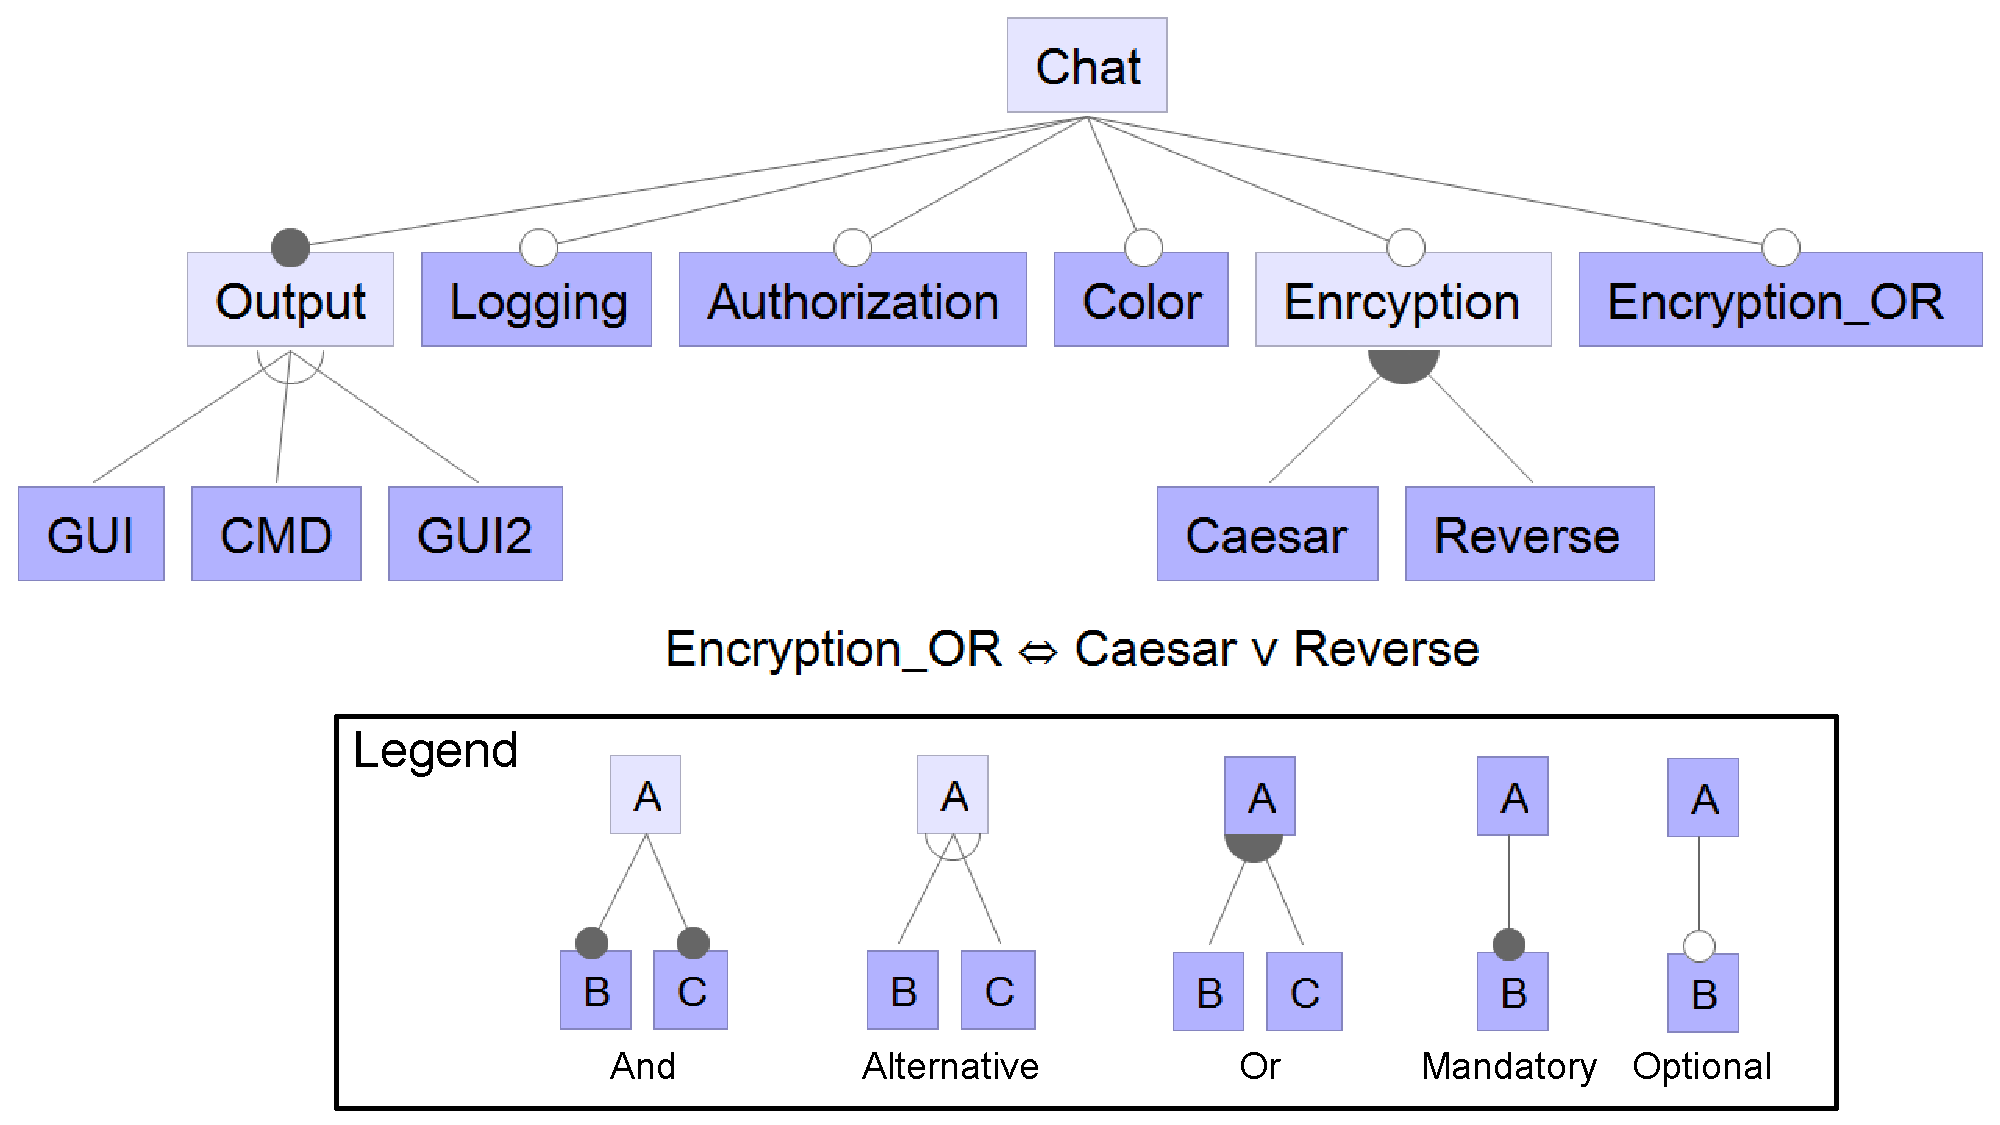
\epsfig{file=image/fm.bmp, width=8.5cm}
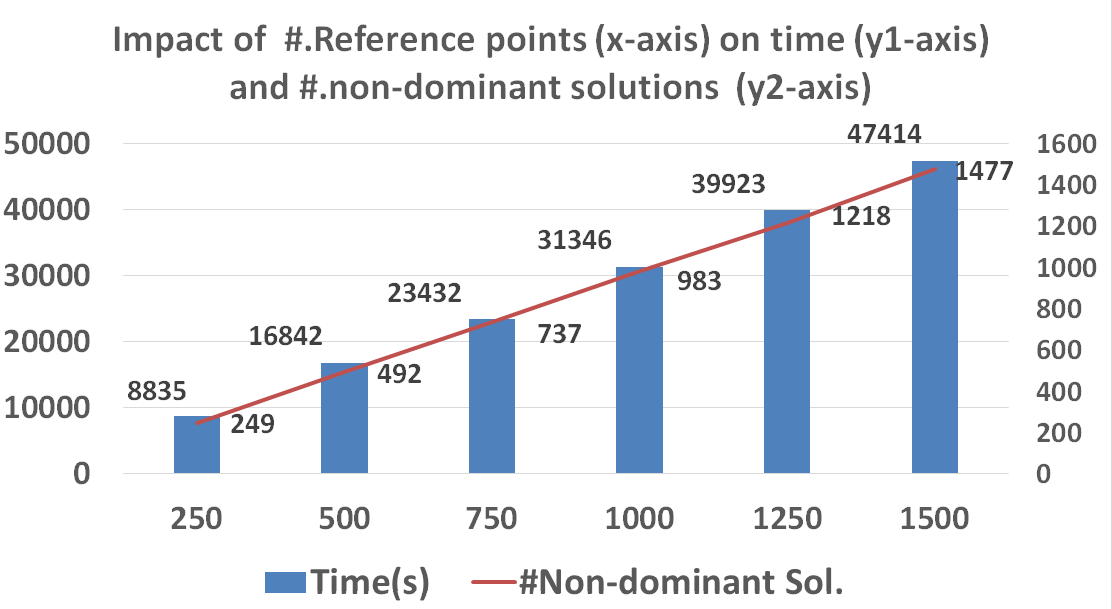
\includegraphics[width= 9cm]{image/rf.png}
\vspace{-6mm}
\caption{Impact of \#. reference points (x-axis) on execution time (y1-axis) and \#.non-dominant solutions (y2-axis) found on \emph{Linux X86 1} }
\label{fig:referPoint}
\end{figure}

%\subsection{Discussion}\label{sec:application:discuss}


\noindent\textbf{Threats to Validity.}
One threat to validity is about randomly generated values for feature attributes (i.e.,  Cost,  Defects,  and  Used  Before). %Due to the difficulty in getting feature attributes  associated with  real-world  products,
To  mitigate  the  effect  of  randomness, we  generate  10  sets  of  attributes for each model. Due to the page limit, we just report 2 or 4 representative attribute sets in the evaluation. According to \cite{DBLP:journals/asc/XueZT0CC016} and our observation, impact of attribute values is minor to the results ---  if on two sets of attributes a method is better; then in general (like on ten sets) this method is better. %Besides, for each set, IBED or IBEA is repeatedly executed for 30 times, and  report  the  medium  values  of the  metrics.
The second threat is about the systems chosen in evaluation. In future, the \emph{EC2}  feature  model \cite{DBLP:journals/fgcs/Garcia-GalanTRC16} and  the  \emph{Drupal} model  \cite{Sanchez2015} need to be included in the evaluation. The last threat is about the parameters of the EAs used as baseline tools. We used the best parameter setting of IBED (and also IBEA) reported by \cite{DBLP:journals/asc/XueZT0CC016}.

\vspace{-2mm}
%\noindent\textbf{Generality of \ourSol.} \ourSol~is proven to be effective and scalable in solving the optimal feature selection in SBSE. We are eager to try out \ourSol~for other MOO problem, as long as the constraints and multiple objectives are linear. As \ourSol~is designed as a general method for MOIP with linear constraints, some existing benchmarks [??] can be used to evaluate \ourSol. We plan to submit \ourSol~to OR community for review.
%\subsection{Heuristic, Analytic or Statistic?}\label{sec:discuss:how}

\section{Related Work}\label{sec:related}

\noindent\textbf{The Optimal Feature Selection Problem.}
White \emph{et al.}~\cite{DBLP:journals/jss/WhiteDS09} first modeled the feature selection problem as a Multidimensional Multi-Choice Knapsack Problem (MMKP), and applied Filtered Cartesian Flattening (FCF) to derive an optimal feature configuration subject to resource constraints.
%The existing works \cite{DBLP:journals/jss/GuoWWLW11,DBLP:conf/icse/SayyadMA13,conf/cmsbse/SayyadMA13,DBLP:dblp_conf/kbse/SayyadIMA13, DBLP:conf/issta/TanXCSLD15} have adopted evolutionary algorithms (EAs) for feature selection with resource constraints and product generation based on the value of user preferences, respectively.
Guo \emph{et al.}  \cite{DBLP:journals/jss/GuoWWLW11} first proposed a genetic algorithm (GA) approach to tackle this problem. In \cite{DBLP:journals/jss/GuoWWLW11}, a repair operator is used to fix each candidate solution, and make it comply with the feature model during evolution. %This approach might be non-terminating, and furthermore, it does not take advantage of the automatic correction  that brought by the GA.
One limitation of \cite{DBLP:journals/jss/GuoWWLW11} lies in aggregating all objectives into a single fitness function with different weights. %This only gives users a solution specific to the weights used in the objective formula.

To address the objective aggregation issue, Sayyad \emph{et al.}~\cite{DBLP:conf/icse/SayyadMA13,conf/cmsbse/SayyadMA13} first proposed to apply various MOEAs, and a range of optimal solutions (a.k.a., a Pareto front) is returned to the user as a result. As reported, IBEA \cite{DBLP:conf/ppsn/ZitzlerK04} yields the best results among the seven tested EAs in terms of time, correctness and satisfaction to user preferences. In \cite{DBLP:dblp_conf/kbse/SayyadIMA13}, they further used static method to prune features before execution of IBEA for reducing search space. They also introduced a ``seeding method\rq\rq{} by pre-computing a correct solution, which was later implanted the initial population of IBEA. Along this line, Tan \emph{et al.} \cite{DBLP:conf/issta/TanXCSLD15} improved these previous studies by using a novel feedback-directed mechanism to existing EAs. %In their approach, the feature model is first preprocessed based on SAT solving to remove the prunable features, before the execution of an EA. %We have shown that we always prune more features compared to the pruning method in~\cite{DBLP:dblp_conf/kbse/SayyadIMA13}.
%During evolution, the violated constraints would be analyzed and analyzed results are used as feedback to guide evolutionary operators (i.e., crossover and mutation) for producing correct offsprings. %for the next round. This feedback-directed mechanism is mainly used to improve the correctness of offsprings.
Similarly, to improve the correctness, Hierons \emph{et al.} \cite{DBLP:journals/tosem/HieronsLLSZ16} proposed the $1+n$ approach that prioritizes the number of failed constraints and considers the correctness objective first.
%Our evaluation has shown that our method produces more promising offsprings (that have fewer violated constraints), which has led to faster convergence and resulted in more valid solutions in a significantly shorter amount of time.
Recently, IBEA (including its variants) is integrated with other techniques for achieving better results.  Henard \emph{et al.}~\cite{DBLP:conf/icse/HenardPHT15}
integrated IBEA with constraint solving. They permuted different SAT parameters to maximize the diversity of SAT solutions in a cheap way by calling SAT solver hundreds of times. %The merit is that the fixing of incorrect offspring of IBEA population via SAT solutions is done during evolution.
Xue \emph{et al.}~\cite{DBLP:journals/asc/XueZT0CC016} integrated IBEA with differential evolution (DE) for achieving both correctness and diversity of solutions. % Their method, named IBED, is a dual-population EA, where two populations are evolved with two different types of EA operators, i.e., IBEA operators and DE operators.

\vspace{0.5mm}
\noindent\textbf{MOO and SBSE.}
Apart from the above problem, MEOAs have exhibited the effectiveness in solving some earlier SBSE problems~\cite{DBLP:journals/csur/HarmanMZ12}. For example,  multi-objective planning for software project overtime is the SBSE problem solved by a variant of NSGAII \cite{DBLP:conf/icse/FerrucciHRS13}. Besides, the problem of bi-objective software effort estimation is also addressed by NSGAII~\cite{DBLP:conf/icse/SarroPH16}.
 In software refactoring, multi-objective refactoring step recommendation via NSGAII helps to ensure the semantic coherence of refactored program~\cite{DBLP:journals/ese/MkaouerKCHD17}. Last, a branch of MOO studies is on software test suite selection, minimization and prioritization~\cite{DBLP:conf/issta/YooH07}\cite{DBLP:journals/tse/MarchettoIASS16}.
NSGAII, which is used in aforementioned studies, is suitable  for  more  spread  out solutions  and  absolute domination. Hence, NSGAII works well if the solution space is not highly-constrained and diversity can help find more solutions. However, for the optimal feature selection, the preference of diversity (using NSGAII) may bring more incorrect solutions (since correct solutions may be concentrated in certain areas of  the solution space). To assure this, IBEA is advocated~\cite{DBLP:conf/icse/SayyadMA13}\cite{conf/cmsbse/SayyadMA13}. %IBEA is also combined with DE to achieve both correctness and diversity~\cite{DBLP:journals/asc/XueZT0CC016}.

%In \cite{DBLP:journals/infsof/HarmanJ01}, Harman \emph{et al.} proposed the term Search-Based Software Engineering (SBSE), and reported that the surveyed and proposed optimization techniques for SE problems by 2001 were all single-objective based. Seeing the potential of using multi-objective optimization, Harman \cite{DBLP:conf/icse/Harman07} discussed about the possible usage of the meta-heuristic search techniques such as: simulated annealing and genetic algorithm. Harman considered it insensible combination of  multiple metrics into an aggregate fitness in the way of assigning coefficients, and further suggested to use Pareto optimality rather than aggregate fitness.

\vspace{0.5mm}
\noindent\textbf{OR and SBSE.} IP has been used for the instantiation of products --- the valid product feature selection problem~\cite{DBLP:conf/splc/Broek10}. In~\cite{DBLP:conf/splc/Broek10}, only one single objective is considered, not addressing MOO via IP. Earlier than this study, requirement interdependencies were resolved via IP\cite{DBLP:journals/re/Carlshamre02}.
Then, flexible release planning was solved by IP~\cite{DBLP:conf/caise/AkkerBDV05}.
Subsequently, requirements selection and scheduling for the release planning were integrated and optimized by IP to cater for budgetary constraints  \cite{DBLP:conf/refsq/LiABD07}. Further,  IP was combined with computational intelligence and human negotiation to address conflicting objectives \cite{DBLP:journals/software/RuheS05}.
Recently, IP is not widely used due to its scalability issues and strict limitation on the application. Meanwhile, due to the emergence of MOO problems in SBSE, MOEAs  become the default method.

 %In 2009, Harman \emph{et al.}~\cite{tr:sesw} reported that MEOAs had been deployed to attain multi-objective optimization (especially two objectives), and the mainly used techniques were NSGA-II and SPEA2. By them, few studies had examined the performance and suitability of the commonly used MEOAs on more than three-objective optimization. In 2010, Bowman \emph{et al.}~\cite{DBLP:journals/tse/BowmanBL10} solved class responsibility assignment problem by applying five-objective optimization techniques on UML model analysis. They reported that SPEA2 can generally attain better results than RMHC1 and RMHC2. Recently, Sayyad \emph{et al.}~\cite{conf/raise/SabouriK11} found that among the existing application of MEOAs, the population based algorithm like NSGA-II was widely chosen for optimization of two or three objectives. Meanwhile, the comprehensive discussion and comparison of the suitability of different MEOAs are absent.
\vspace{-2mm}

%\input{relatedOld}
%\vspace{-1mm}
\section{Conclusion}\label{sec:conclusion}
In this paper, we formulate the optimal feature selection problem in SBSE as a MOIP model. Different from all previous studies that adopt MOEAs, we seek to apply MOIP methods. We try the \naiveSol~and CWMOIP, and prove the completeness of their solutions on small systems. However, they are not scalable. To address this, we propose an innovative MOIP method --- \ourSol. Evaluation shows that \ourSol~is scalable and finds significantly more non-dominant solutions than IBED in most cases, using similar or less time. In future, we will apply \ourSol~to more suitable SBSE problems.

\newpage

\bibliographystyle{ACM-Reference-Format}
\bibliography{section/reference}

\end{document}
